\documentclass[a4paper]{report}

\usepackage[english]{babel}
\usepackage[T1]{fontenc}
\usepackage[utf8]{inputenc}
\usepackage{amsmath}
\usepackage{graphicx}
\usepackage{pifont}
\usepackage{hyperref}
\usepackage{listings}
\usepackage[section]{placeins}
\usepackage{fancyhdr}
\usepackage[usenames,dvipsnames,svgnames,table]{xcolor}

\title{Genomizer}

\author{You}

\date{\today}

\fancyfoot{}
\fancyhead[RO,LE]{\thepage}
\fancyhead[LO]{\leftmark}
\fancyhead[RE]{\rightmark}

\begin{document}

\pagestyle{fancy}
%\maketitle

\title{Tidsrapport \\ 
	Programvaruteknik \\5DV151\\
	VT-14 }
	\begin{titlepage}
		\thispagestyle{empty}
		\begin{large}
			\begin{tabular}{@{}p{\textwidth}@{}}
				%\textbf{\hfill \today} \\
				%\textbf{2014} \\
			\end{tabular}
		\end{large}
		\vspace{35mm}
		\begin{center}
			\Huge{\textbf{Technical documentation}\\ Genomizer} \\
			\vspace{10mm}
			\LARGE{Version 2.0} \\
           \vspace{5mm}
           
            Publication date: 5/12/2014 \\
            

			\vspace{70mm}
            
			\begin{normalsize}				
		 %
         %
         %	
			\end{normalsize}
		\end{center}
	\end{titlepage}

%\begin{abstract}
%Your abstract.
%\end{abstract}

\makeatletter
\renewcommand\paragraph{%
   \@startsection{paragraph}{4}{0mm}%
      {-\baselineskip}%
      {.5\baselineskip}%
      {\normalfont\normalsize\bfseries}}
      
\renewcommand\subparagraph{%
   \@startsection{paragraph}{4}{0mm}%
      {-\baselineskip}%
      {.5\baselineskip}%
      {\normalfont\normalsize\bfseries}}
\makeatother

\lstdefinestyle{customc}{
  belowcaptionskip=1\baselineskip,
  breaklines=true,
  frame=L,
  xleftmargin=\parindent,
  language=C,
  showstringspaces=false,
  basicstyle=\footnotesize\ttfamily,
  keywordstyle=\bfseries\color{green!40!black},
  commentstyle=\itshape\color{purple!40!black},
  identifierstyle=\color{blue},
  stringstyle=\color{orange},
}

\lstdefinestyle{customsh}{
  belowcaptionskip=1\baselineskip,
  breaklines=true,
  frame=L,
  xleftmargin=\parindent,
  language=C,
  showstringspaces=false,
  basicstyle=\footnotesize\ttfamily,
  keywordstyle=\bfseries\color{green!40!black},
  commentstyle=\itshape\color{purple!40!black},
  identifierstyle=\color{blue},
  stringstyle=\color{orange},
}

\newcommand{\appName}{\textit{Genomizer}}
\newcommand{\addImage}[1]{\centering\includegraphics[width=\textwidth, keepaspectratio=true]{#1}}
\newcommand{\addScaledImage}[2]{\centering\includegraphics[scale=#1]{#2}}
\newcommand{\addImageVertical}[1]{\centering\includegraphics[height=\textwidth, angle=90, keepaspectratio=true]{#1}}
\newcommand{\addScaledImageVertical}[2]{\centering\includegraphics[scale=#1, angle=90]{#2}}
\newcommand{\refer}[1]{\autoref{#1}}
\newcommand{\addCode}[3][c]{\lstinputlisting[caption=#3, escapechar=, style=custom#1]{#2}}
\newcommand{\filePath}[1]{\texttt{#1}}
\newcommand{\click}[1]{\ding{43} \textbf{\textit{{#1}}}}
\newcommand{\term}[1]{\textit{#1}}

\newcommand{\userstory}[2]{
\begin{tabular}{|l|}
\hline
\\
{\large \textbf{#1}} \\ \hline
\\
\begin{minipage}{\textwidth}
#2
\end{minipage}
\\ \hline
\end{tabular}
}

\setcounter{secnumdepth}{5}

\setlength{\parindent}{0pt}
\setlength{\parskip}{10pt}

\graphicspath{ {figures/} }

\tableofcontents

\chapter{Introduction}
% When conducting experiments and analyzing data within the epigenetics field, a large amount of data is generated. This data needs to be handled and stored in an easy, secure and efficient way. Analyzing this data is today a very time consuming task, involving several manual steps with little to none user friendliness. These steps might also change and/or be replaced. A system for analyzing and storing epigenetics data safely and efficiently in a single application does not exist today. 

% Within the PVT Project we are developing a system that addresses these issues. The system is built for experienced epigenetic scientists as well as for new users. This system focuses on making analyzing and storing epigenetics data less time consuming and more efficient by gathering these tasks in one common application and by using a database for storing. The system will help users to easily search the database for data. Data from the database could either be used for analyzing just by marking what data to be used or to be downloaded to a local space in a wide variety of different file formats. The database is accessed from multiple devices (Windows, Linux, OSX, Android and iPhone) using separate client applications. 

\appName\ is a system for storing and analyzing \term{DNA}-sequences. It was designed for researchers in the field of epigenetics, who are interested in where on a \term{DNA} string a certain protein bind. In order to get this information, experiments are conducted and \term{raw} data files collected. These data files are then converted, in a series of steps, to files suitable for analysis. \appName\ allows the researchers to upload \term{raw} files to a server and automate the generation of analysis data. 

\appName\ is developed by the students of a course in software engineering at \term{Umeå University}. This documentation is directed towards three main groups. The first group are the users that wants to use the software. The second group are the system administrators that wants to maintain the system and help other users with more advanced tasks. The third and final group are system developers that wishes to expand and improve the current software.

The first part of this documentation describes the target group of the software. This is followed by instructions of how to use the software for the common user. Then a chapter follows with instructions of how to deploy the server together with the software. This chapter is directed towards administrators and developers. After these initial chapters that is focused on using the system follows chapters with more indepth information on how the software is designed and implemented. 

% Finally at the end of the documentation are appendixes that helps describe different parts of the software and the software development.

\chapter{Target group and needs}
To understand who this system is built for and what it needs to do, the following chapter will explain the target group and its needs.

\section{Target group}

The main group that wants to utilize the \appName\ system is the researchers at \term{Epigenetic Cooperation Norrland (EpiCoN)}. They are conducting experiments on \term{DNA} and proteins to see where proteins bind to the \term{DNA} strings. This information combined with knowledge about the location of genes within a given genome, will give the researchers a hint of which proteins are active in enabling and disabling genes. These results are important in the study of how cells remember which genes should be enabled after cell division.

The data files retrieved from experiments are manually handled by the researchers and they have written scripts to process \term{raw data} to \term{profile data}. In this process they are using the program \term{Bowtie} to unscramble the \term{DNA} data. An other program that is used to manipulate experiment data is the program \term{LiftOver}, used to adjusting results to a different genome release.

The researchers at \term{EpiCoN} have varying computer skills. While they all have basic computer knowledge not all are familiar with more advanced computer tasks, such as running scripts at command line level. The researchers that have less computer knowledge becomes dependent on the ones who do. The researcher that has the knowledge to use all the scripts and software can perform the tasks they and other researchers need, but these tasks are very time consuming.

Students at \term{Umeå University} sometimes have the need to look at research done by \term{EpiCoN}. These students doesn't have the same trust to handle the research as the main staff at \term{EpiCoN}.

Their main field of knowledge lies within epigenetics. It is an international group with many different native languages, which means that they mainly use english to communicate.

%Since biologists have varying experience with software and software development, the system will be designed to be as user friendly as possible. The international language of science is english, therefore the entire product shall be in english (both the product and its documentation). Since target audience has different knowledge in biology, the product and its functions shall be simple, self explanatory and have an interface. The biology students are not as trusted as the standard users and therefore their data access will be restricted in some way. The system might also have some administrators. An administrator primarily handles new users and user rights. If the system expands the administrator may also have to maintain the system. For starters some of the biologists with more computer knowledge will be given authority to handle users and user rights.

\section{Client needs}
This target group of researchers from \term{EpiCoN} needs a system to structure the big amount of genetic data that they use daily. The data is used for research of cell memory, how cells remembers which sequences in the \term{DNA} that should be active after cell division. 

There are mainly three data types used for this research and that the system should handle: \term{raw data}, \term{profile data} and \term{region} data. \term{Raw data} is the raw output from an experiment and isn't used much for actual studies. Rather it's processed to \term{profile data}. \term{Profile data} describes the amount of reads found for every base pair in an organism's genome. \term{Region data} is further processed \term{profile data} consisting of regions where every basepairs read strength is above a given threshold and fault tolerance. The region gets a value based on the average of the base pair reads for the given region.

\subsection{Storage}
Most importantly the researchers want a central secure location to store their genome data in a structured  way so that it is easy to find the data the researchers are looking for when doing research. By having a central location for genome data the researchers can more easily collaborate than they do today. The researchers want the database to be locked down from outside access and that the data is stored in a secure way to avoid loss of data. Data integrity is of great importance, data must not change or become corrupt in the database.

\subsection{File formats}
As different software uses different file formats for genome data, and the tools for converting files between these file formats are not very user friendly, converting between file formats is a time consuming process for the researchers.  The researchers want this work to be carried out by the system.

\subsection{Genome release}
From time to time a new genome release is released for genome data for a specific species. The researchers needs a way to convert between these releases. Errors in a release can be discovered after publication. It is therefore important to keep data files that are compatible with an older release for some time after a new release is published.  

\subsection{Analysis}
The researchers want to do some analysis on the server. Some analysis is to combine regions using logical arithmetic and in such a way construct new regions. It should also be possible to create new regions from a reference point. Another interesting analysis is overlap analysis which shows how much a number of genome experiments overlap.

\subsection{Visualization}
To be able to review the results from doing analysis on data,  the researchers want a graphical presentation of the results.

\chapter{Service description}
This chapter will present an overview of the services that the \appName\ system will provide. 

\section{Usage}
The service will a central database which can be accessed from multiple devices (Windows, Linux, OSX, Android and iPhone) using different clients. Using the desktop clients, users can upload genome data and annotate it with info about the data.   

Advanced searches or different annotation can be performed in the database to find data which has previously been uploaded to the database. When some interesting data is found in the database it can be downloaded in a variety of file formats. If a file does not exist in a specific file format it will be converted before it's sent to the user.

\section{Genome release}
The researchers will be able to upload chain files between different genome releases and genome references for different species. When a chain file is uploaded it will be possible to convert profile and region data between different releases.

\section{Analyze}
The user will be able to conduct different types of analysis on different datasets, the actual analysis will be calculated on the server to avoid heavy workload on the clients.

\section{Visualization}
The system will have support for opening a session in Integrated Genome browser directly from the interface.

\section{Workspace}
To gather, organize and share data the concept workspace has been introduced. A user can save raw data, profile data and region data as well as analysis results in a workspace. The workspace is saved on  the server so that the user can continue their work on another place as long as internet is available.  Another feature with workspaces is that it can be shared between users, this is valuable when users work on different locations.

\section{Mobile}
In the mobile application the users will be able to start downloading new datasets from other databases to the genomizer database, start or schedule processing of data and view the visualization of analysed data.

\chapter{User manual}
%User manuals for the different clients. Directed towards users (includes everyone). Start with subsection here.

%This chapter explains to the user how each client should be used. It starts with the desktop and web clients. These clients are the main clients that can handle the main features. Then comes instructions for the mobile clients that are designed to search for files and tell the server to convert them.

This chapter explains how you use each of the \appName\ clients. First instructions on how to use the desktop and the web clients are presented. These are the clients which provide the most functionality. The mobile clients are more lightweight and offer a subset of the functionality presented by the desktop client. Instructions on using the smartphone applications for \term{Android} and \term{iOS} are presented in their on sections at the end of the chapter. 


\section{Desktop}
This is a user manual for the desktop client. It will provide guides on how to use the client and the different functionalities it holds. The screenshots shown in this document are made from a Linux machine, but the Desktop application also runs on Windows or Mac, and will follow the design priciples thereafter. Because of this, the look of the client may vary, but the functionality is the same, and hopefully this manual will be of service anyways. 

\subsection{Login and startup}
When you start this application the first thing that's displayed is a login screen, as illustrated in \refer{fig:des_login-pic}. In this screen you enter your username, password and the IP-Address for the server and then press login to enter the Genomizer Desktop.

\begin{figure}[htb]
	\addScaledImage{0.5}{des_loginpicture.png}
	\caption{Screenshot of the login screen.}
	\label{fig:des_login-pic}
\end{figure}
The application is built with tabs, as illustrated below in the upper part of \refer{fig:des_desktop-view}. Each tab contains separate features of the application. There are six tabs: Search, Upload, Process, Workspace, Analyze and Administration.
\begin{figure}[htb]
	\addImage{des_searchtab.png}
	\caption{Illustration of the different tabs of Genomizer Desktop and displaying the Search tab.}
	\label{fig:des_desktop-view}
\end{figure}
\FloatBarrier

\subsection{Search}
The first tab that meets the user after logging in is the Search tab, illustrated in \refer{fig:des_desktop-view}. The Search tab uses the same query building technique as the “Pubmed Advanced Search Builder”. It has one text field where you either can type in the query yourself or you can use the query builder below it. Each row in the query builder has at most five components. These are a logical expression, an annotation name field, a free text field or a drop down menu to insert search words, a minus button and a plus button. The minus button removes a row and the plus button adds a row. These buttons are however not available in each row. The plus button is only available in the last row. The minus button is available in every row except if there is only one row in the query builder. The logical expressions combines the annotations, so they are available in every row but the first.
By writing in the annotation text field or selecting a value in the drop down menu you can specify the query the row will produce. Together each row builds a full query. As illustrated in \refer{fig:des_search-query} below.
\begin{figure}[htb]
	\addImage{des_searchtab.png}
	\caption{Illustration of a query, made by the query builder.}
	\label{fig:des_search-query}
\end{figure}
\FloatBarrier

\subsection{Upload}
If the user needs to upload a file to the database it can be done through the upload tab.
When the tab is pressed the user gets presented with a text field and a button where they can search for an existing experiment to upload to and another button for adding a new experiment. When the user presses the new experiment button, the user is presented with annotations they can choose between. If they pressed the existing experiment button, they are instead presented with annotations they can't choose between. They are also presented with buttons named Select files and Upload selected files, with which the user can choose a file via a file browser and upload them. The upload tab is illustrated in \refer{fig:des_upload-view} and the file browser is illustrated in \refer{fig:des_upload}.
\begin{figure}[htb]
	\addImage{des_uploadexisting.png}
	\caption{Illustration of the upload tab where the browse and upload functions are shown.}
	\label{fig:des_upload-view}
\end{figure}

\begin{figure}[htb]
	\addScaledImage{0.4}{des_uploadselect.png}
	\caption{Choosing a file for uploading}
	\label{fig:des_upload}
\end{figure}
\FloatBarrier

\subsection{Process}
In the process tab there is a list called Files that on the left side of the tab. From this list the user can mark RAW-files and choose to create profile data. By left clicking on the files they will be marked. If the user left clicks once again on the same file it will be unmarked. If the user then presses the Create profile data button which is visable in the middle of the tab see \refer{fig:des_process-view}, all the files that are marked will now be processed to profile data. This list of files will be empty unless the user has chosen to process selected RAW-files from the workspace tab. If that is the case then those selected RAW-files will then be visable in the list of files in the process tab. When the user has selected some RAW files the user has the option to change conversion parameters that is above the create profile data button as illustrated in \refer{fig:des_process-view}. These parameters has pre-set values. The conversion parameters are Flags, Genome release files, Window size,Smooth type,Step position,Step size,Print mean and Print zeros. If the user has selected some RAW-files and pressed the Create profile button, then if all went well and the server could convert the files a message "The server has converted: filename" will print in Convert Files for each file that was converted to profile data. If for some reason the server couldn't create profile data for any RAW-file another message "WARNING - The server couldn't convert: filename" will print in Convert Files that is visible in the middle bottom of the process tab see \refer{fig:des_process-view}.


\begin{figure}[htb]
	\addImage{des_processtab.png}
	\caption{Screenshot of the process tab in the program.}
	\label{fig:des_process-view}
\end{figure}
\FloatBarrier

\subsection{Workspace}
The Workspace View is the heart of the application for the user. Chosen files from the search is collected in this view, and the user can choose different options to process and analyze the data. 
For now, the only function here that is implemented is Download, but more will come.
\subsubsection{Download}
The user can make the choice to download. If the user presses the DOWNLOAD SELECTED button seen in \refer{fig:des_workspace-view}, then a pop up menu will present it self to the user as illustrated in \refer{fig:des_download-view}. In the pop up menu, the files that were selected in the workspace will be shown, then the user can choose a file format for each of the files (this functionality is not yet implemented). If the download button is pressed, the user gets to choose a directory where the files will be saved. When a directory has been chosen, the files get downloaded and saved in folders named after the experiments in which they belong. 
\begin{figure}[htb]
	\addImage{des_workspaceselect.png}
	\caption{Screenshot of the workspace tab in the program.}
	\label{fig:des_workspace-view}
\end{figure}
\begin{figure}[htb]
	\addImage{des_download.png}
	\caption{The download files pop up menu}
	\label{fig:des_download-view}
\end{figure}
\FloatBarrier

\subsection{Administration}
The system administration tools for the desktop client is available under the Administration tab. When a user selects the add button in the sidepanel a new popup windows appears. It is possible to write the name of the new annotation and name of new categories in this popup, as well as check a forced annotation box. See \refer{fig:adm_desktopgui}.
\begin{figure}[h!]
\addImage{des_addAnnotation.png}
\caption{The add new annotation popup.}
\label{fig:adm_desktopgui}
\end{figure}

\FloatBarrier

\section{Web}
To access the web application, navigate to a domain and directory that publicly serves the web page. An example of this is the “official” test enviroment: www8.cs.umu.se/~oi11lsm/app/.
All functionality of the web application is (or rather should be) fairly self-explanatory and intuitive. A short description and explanation will be given for each component that have been implemented so far.
\subsection{Using the interface}
This section will describe how to use the interface and how to interact with it.
\subsubsection{Start view}
%figure 2
\begin{figure}[h]
\centering
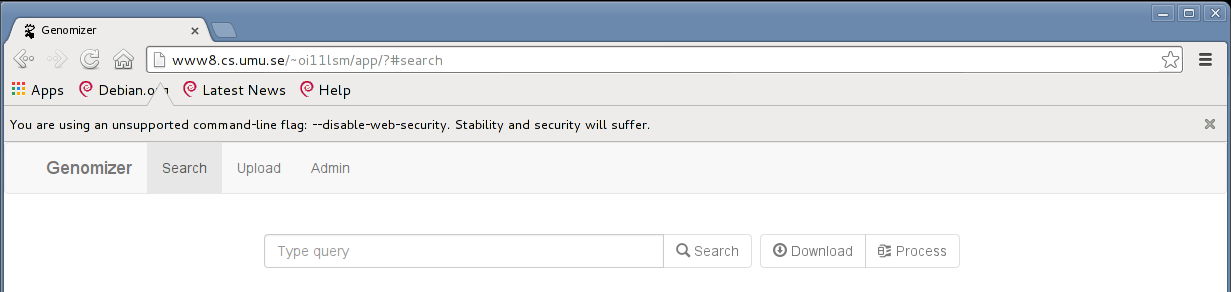
\includegraphics[width=1\textwidth]{web_search_welcome.png}
\caption{\label{fig:web_search_welcome} The welcome screen of the webpage.}
\end{figure}

When the website has loaded, the user is taken to the search page as shown in \refer{fig:web_search_welcome}.

The navigation bar at the top has three buttons with the following functionality:
\begin{itemize}
	\item Clicking the “Genomizer” logo should take the user right back to the start view.
	\item The “Search” button will bring up the search view where the user can enter search strings to be sent to the server, and view search results.
	\item The “Upload” button will bring up the upload view where the user can select files to be uploaded and input annotation to a new experiment.
	\item The “Admin” button will be shown for administrators, that is where the administrator can handle users and annotations.
\end{itemize}
This navigation bar is persistent through all subpages and can easily be accessed.

Below the navigation bar a “search-and-functionality” bar is visible, there is a search field and there are three buttons, Search, Download and process. However, when first entering the page the buttons will be disabled. When you enter something in the search field the search button will become enabled and clickable. 
When the user wants to search for something he can simply write a search query in pubmed style(ex; Exp1[ExpID]) in the search field and either press enter or click the Search button. 

%figure BILD
\begin{figure}[h]
\centering
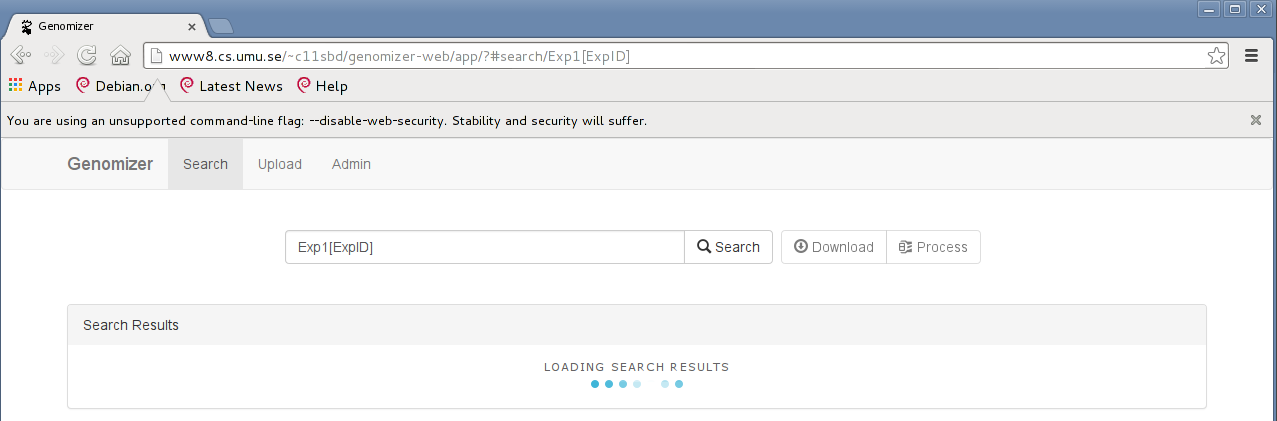
\includegraphics[width=1\textwidth]{web_search_searching.png}
\caption{\label{fig:web_search_searching}will be shown while searching for data in the database before any results are found.}
\end{figure}

After having typed a query and pressed search, the search results will load displaying the loading spinner as can be seen in figure \refer{fig:web_search_searching}.
%figure x3
\begin{figure}[h]
\centering
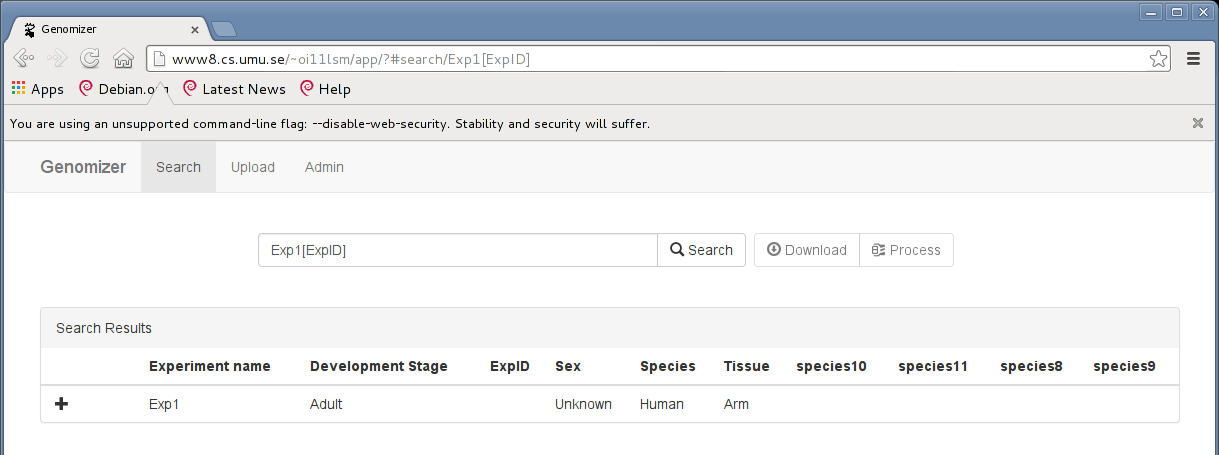
\includegraphics[width=1\textwidth]{web_search_searchTab.png}
\caption{\label{fig:web_search_searchTab}the search tab after a search for ‘Exp1[ExpID]’.}
\end{figure}

The view shown in \refer{fig:web_search_searchTab} contains two major elements; a “search-and-functionality” bar and a list of search results retrieved after searching for ‘Exp1[ExpID]’. The buttons next to the search bar are supposed to do what they say: 
\begin{itemize}
	\item “Search” searches for the query in the search bar. 
	\item “Download” downloads the selected files. 
	\item “Process” brings up a new window in front of the search view with options for file processing. This feature is demonstrated further in Figure \refer{fig:web_process_modal}.
\end{itemize}

Below the search bar in \refer{fig:web_search_searchTab} is the “search results” list. This list contains all experiments returned from a search. Every experiment can be expanded to show the file types it contains,. Each file type can be expanded to show all files of that type in the experiment. Each file has a check box next to it that is used to select files to be processed or downloaded, currently the user is only able to select one file at a time. 
%figure x4
\begin{figure}[h]
\centering
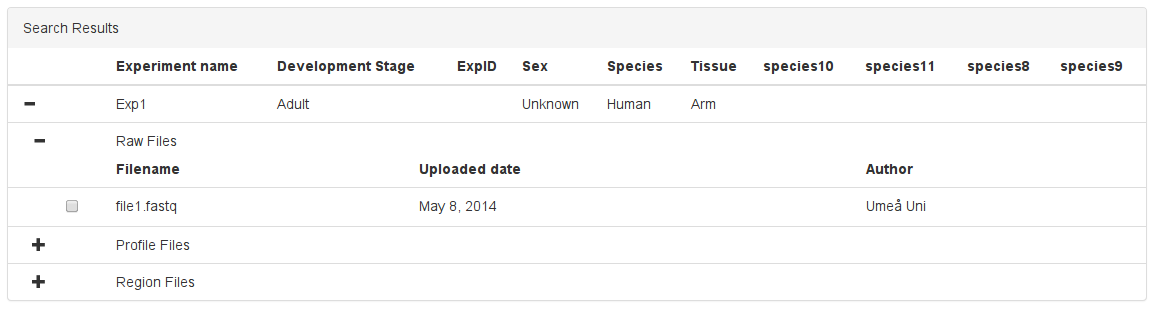
\includegraphics[width=1\textwidth]{web_search_searchResult.png}
\caption{\label{fig:web_search_searchResult}the search results table zoomed in, displaying a raw file’s information after having expanded an experiment.}
\end{figure}

If a search is successful, you will be met with a table of results. This table has a header displaying the annotation types. Below that, all the experiments returned from a search and their corresponding annotation values, as can be seen in \refer{fig:web_search_searchResult}.
%figure BILD PÅ NO SEARCH RESULTS
\begin{figure}[h]
\centering
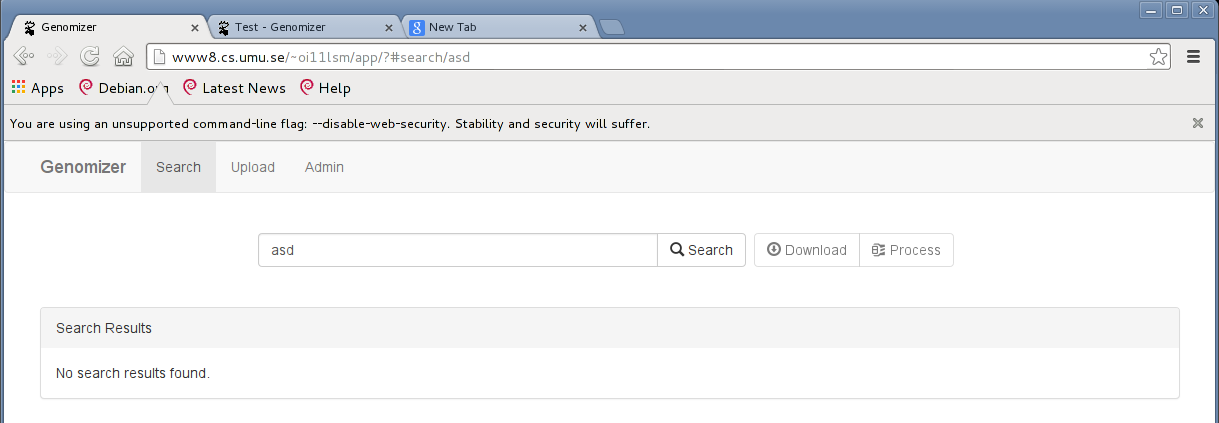
\includegraphics[width=1\textwidth]{web_search_noResult.png}
\caption{\label{fig:web_search_noResult}tells the user that no data was found given the search query entered by the user.}
\end{figure}

If the search is unsuccessful, the Search Results table will be empty stating “No search results found” as can be seen in \refer{fig:web_search_noResult}.

\subsubsection{The processing modal}
%figure X6
\begin{figure}[ht]
\centering
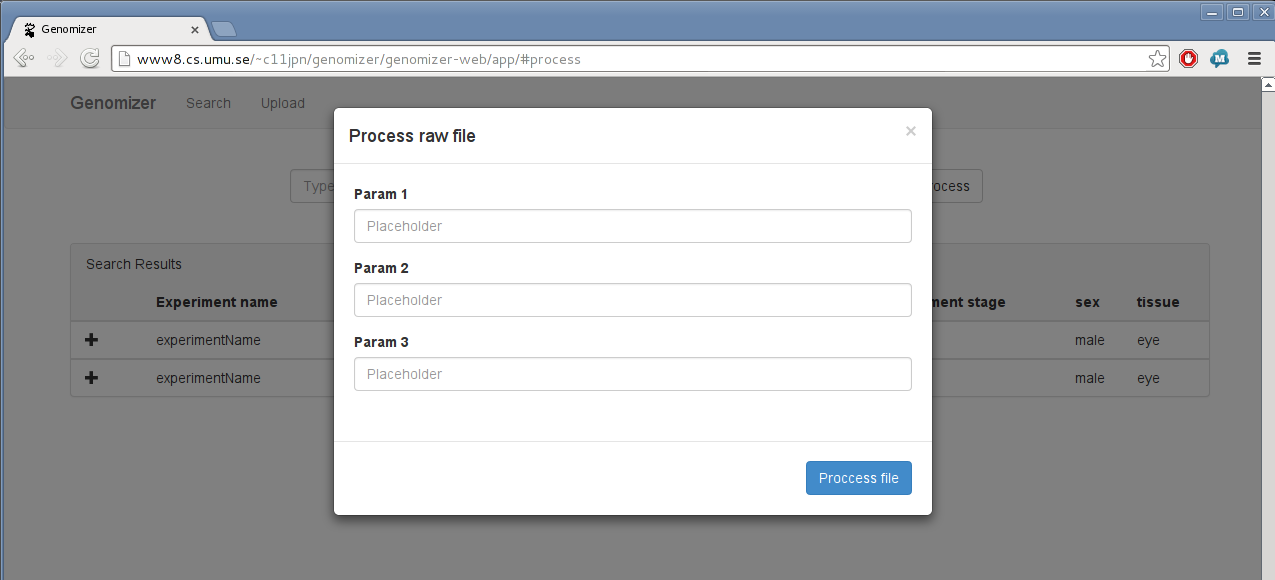
\includegraphics[width=1\textwidth]{web_process_modal.png}
\caption{\label{fig:web_process_modal}The process file modal.}
\end{figure}

The user will be presented with the view in \refer{fig:web_process_modal} when he wants to process one raw file to profile data. The user will already have selected one file he wishes to process and he will enter the parameters for the processing.
\subsubsection{The upload view}
%figure X7
\begin{figure}[h]
\centering
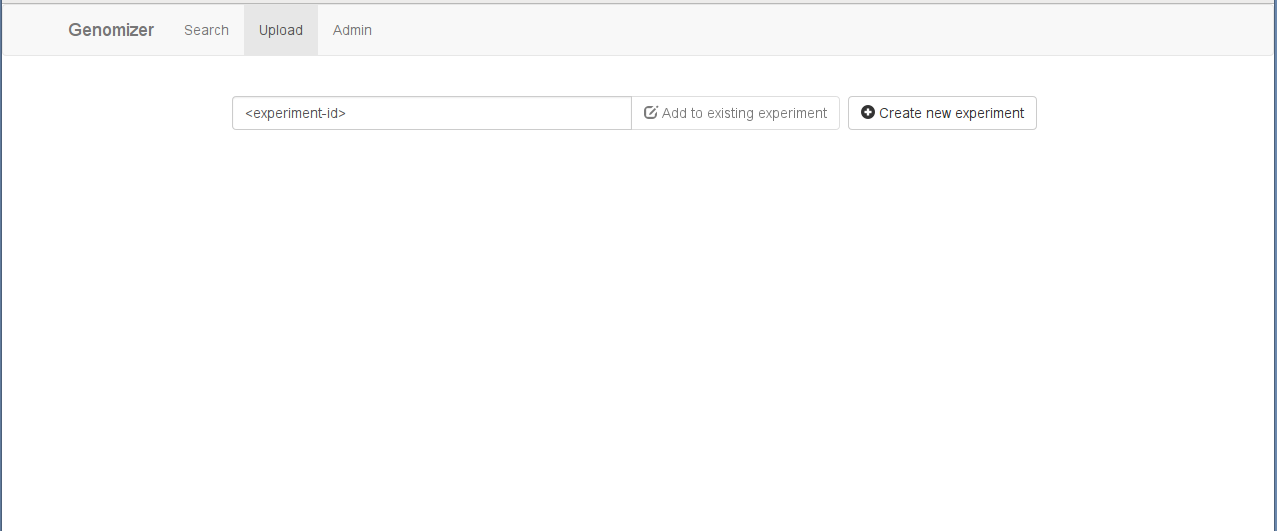
\includegraphics[width=1\textwidth]{web_upload_uploadView.png}
\caption{\label{fig:web_upload_uploadView}The upload view.}
\end{figure}

When the user presses the upload tab in the navigation bar the view in \refer{fig:web_upload_uploadView} will appear. The user has the option to create a new and fresh experiment or to load an existing experiment by entering its experiment ID. 
%figure X8
\begin{figure}[h]
\centering
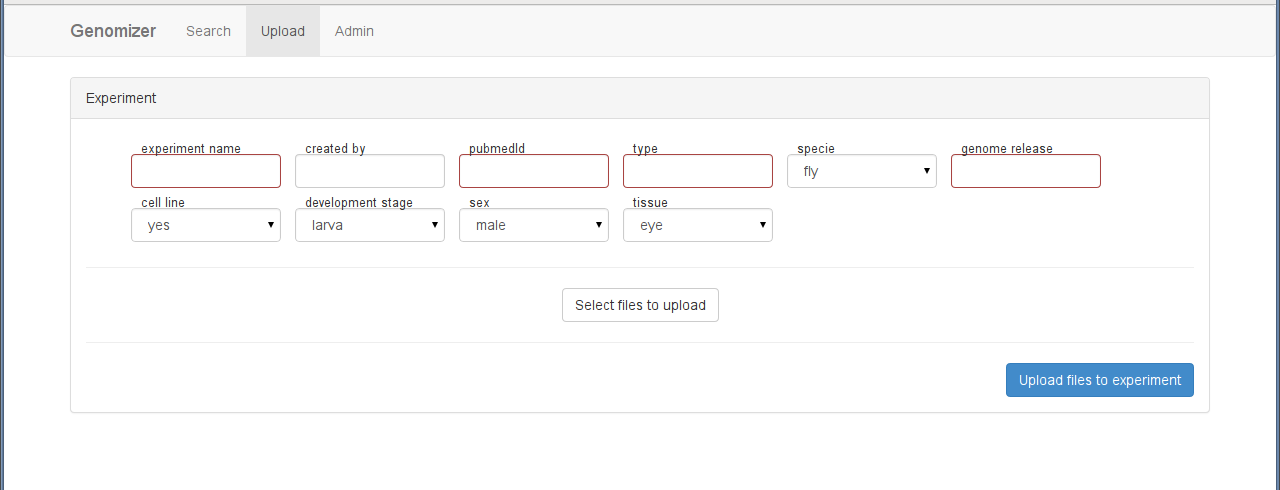
\includegraphics[width=1\textwidth]{web_upload_newExperiment.png}
\caption{\label{fig:web_upload_newExperiment}Creating a new experiment.}
\end{figure}

After clicking the “Create new experiment” button the view in \refer{fig:web_upload_newExperiment} will appear. Here the user can input the annotations for the experiment through either freetext fields or drop-down lists. If a freetext field has a red border around it, that annotation is required and no files can be uploaded before it has been filled in. The user can also browse for local files to upload by clicking the “Select files to upload” button. 
%figure X9
\begin{figure}[h]
\centering
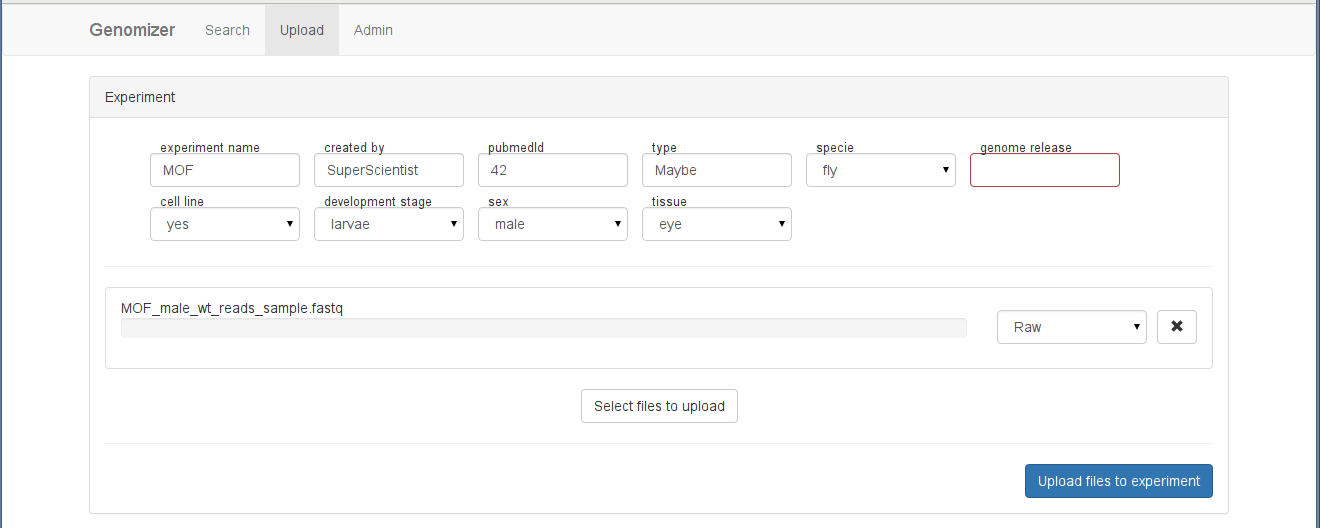
\includegraphics[width=1\textwidth]{web_upload_fileUpload.png}
\caption{\label{fig:web_upload_fileUpload}File selected for upload.}
\end{figure}
 
When the user has selected files, they will appear below the annotations as in Figure \refer{fig:web_upload_fileUpload}. The file’s name is displayed in the top left corner. On the right side there is an option to select what type of file is being uploaded and an option to remove the file from the experiment.

When the user is done selecting files and annotations it can click the “Upload files to experiment” button. The files will then be sent to the server with the specified annotations (this functionality might not be fully working by the time this was written).

\subsubsection{Systemadministration view}

This part of the web application is only accessible if the user have administrator-rights. It is integrated with the rest of the web UI and accessible through an admin-tab. The administrator can through this site see all existing annotations, add new annotations and delete existing ones.
The startpage of this section has a Create new annotations button, a list of existing annotations in the database and an edit button per existing annotation. 
The view currently looks like in figure \refer{adm__web_annotationView}. 

\begin{figure}[h]
 \addImage{web_sysadminAnnotationView.jpg}
 \caption{The startpage for the administrator in the web client}
 \label{adm__web_annotationView}
\end{figure}

For each annotation in the annotations list, an Edit button is available. 
When pressed, it will take you to a page in which you can edit the selected annotation to change its name, 
type and whether it is forced (See \refer{adm_web_editView}). 

\begin{figure}[h]
 \addImage{web_sysadminEditView.jpg}
 \caption{The edit annotation view}
 \label{adm_web_editView}
\end{figure}
\newpage
In the edit page the admin can see the attributes of the chosen annotation and is able to delete the chosen annotation.

If the admin clicks on Create new annotation from the admin startpage, another view will open with the following structure:
\begin{itemize}
 \item Annotation Name
 \subitem Admin can enter a name for the annotation
 
 \item Annotation Types
 \subitem Yes/No/Unknown - this will create a drop-down list with those three options.
 \subitem Freetext - will create an annotation that the users will be able to enter anything.
 \subitem Drop-down list - will enable a fourth field enabling the admin to enter which items that this list will contain.
 
 \item Forced Annotation
 \subitem Admin can choose if the new annotation should be forced for users to enter. 
\end{itemize}

A Create Annotation will, if all necessary information has been entered, result in the annotation to be added to the database. Otherwise the admin will be alerted of the mistake and nothing will be created.
\newpage
A back button which takes the user back to the annotations start page is also available in this view. In figure \refer{adm_web_createView} the create annotation view can be seen.

\begin{figure}[t]
 \addImage{web_sysadminCreateAnnotation.jpg}
 \caption{The view for administrators where new annotations can be created}
 \label{adm_web_createView}
\end{figure}

\subsection{Setting up the application}
To setup the application, move the content of the folder called app in genomizer-web to the desired location from where the application should be run. To run the webpage open a web browser and enter the url to the folder which contains the \texttt{index.html} file(where the content of app was placed).
Ex. given that the genomizer-web folder is placed in my home folder and i want to put the webpage in a folder called public\_html which is also in my home folder. In linux i do the following steps.
\begin{enumerate}
	\item Navigate to the app folder: \texttt{“cd ~/genomizer-web/app/”}
	\item Move the contents of app to the folder called public\_html:\\ \texttt{“mv * ~/public\_html/”}
	\item Given that the url to the pubilc\_html folder is: \\ \filePath{“www8.cs.umu.se/~c11abc/”}
	\item To run the application start a web browser and type \\ \filePath{“www8.cs.umu.se/~c11abc/”}
\end{enumerate}
This will open the webpage in the browser.

\FloatBarrier

\section{Android}
In this section you will find instructions for the usage of the Genomizer android application. \ref{sec:and_start} describes how to start the application and \ref{sec:and_search} gives instructions on how to search for experiments.
\subsection{Start the application}\label{sec:and_start}
Localize the Genomizer icon in the android view of all your installed apps or
use a shortcut on one of your \term{desktop views}. Click the icon in order to start
Genomizer, you will be presented with the login screen.

To start working with your Genomizer app you have to login. If you have a
account with the service: insert your user name and password in the correspond-
ing boxes and press \click{Sign in} to access the application. If you are not yet
registered with the service, ask the system administrator for help with
the creation of your account.
\subsection{Search for files}\label{sec:and_search}
The search view offers a way to find data files with certain attributes. This view is accessed directly after logging in and can be reached at any time by pressing the
search icon on the action bar.

The annotation text fields can be filled in to find files matching the search
criteria. By checking the check box to the right of the annotation field, it gets
activated and appended as part of the search criteria. The functionality can
be used to conduct many similar searches by adding and subtracting criteria as
requested. The search is initiated by pressing \click{Search} at the bottom of the
page.

After pressing Search you will be  redirected to the search results view  that displays a list of available experiments that matches the search annotations. Every experiment is listed showing the experiment name. To receive more information about data files that are available for each experiment, click on an experiment in the list. By clicking an entry you will be taken to a new view displaying all available data files for that experiment. The data files are organised by: raw data, profile data and region data. Every data file got a checkbox next to it.  The checkboxes can be used to select files for conversion. When all files are selected click the \click{Send to conversion} button.

\FloatBarrier

\section{iOS}
In order to use the program import the project from github into Xcode from the following repository:
\url{https://github.com/genomizer/genomizer-iOS.git} 

\begin{figure}[ht]
\addScaledImage{0.2}{ios_login.png}
\caption{The login screen.}
\label{fig:ios_login}
\end{figure}
\FloatBarrier

To compile and run the program press \click{cmd+R}. A simulator will start and the login screen will be shown as seen in \refer{fig:ios_login}  below. A user gets logged in when accepted credentials are entered in the \term{username} and \term{password} fields and the \click{Sign in} button is pressed. If incorrect credentials is entered, a popup message is shown, informing the user that the username or password is incorrect.

\begin{figure}[ht]
\addScaledImage{0.2}{ios_search.png}
\caption{The search screen.}
\label{fig:ios_search}
\end{figure}
\FloatBarrier


After logging in, the user is presented with a search view as seen in \refer{fig:ios_search}. The bottom menu bar is used to navigate between the Search-, Selected files- and More-view according to Apples current GUI standards for iOS 7. In the current state, the More-menu only contains a logout button which is used to log out.The Selected files-menu contains a list sorted on file type of files selected by the user. In the search view, the user can search the database for results matching any number of search criteria. To be able to modify the search quickly, a toggle button is available in the rightmost edge of each search field which enables or disables each search field. For example, if the user wants to search for files matching a certain Experiment ID, the user clicks on \click{Experiment ID}, enters the ID and clicks on the toggle button. 


\begin{figure}[ht]
\addScaledImage{0.2}{ios_advSearch.png}
\caption{The advanced search screen.}
\label{fig:ios_advSearch}
\end{figure}
\FloatBarrier

In top rightmost corner there is a button for opening a advanced search view as seen in \refer{fig:ios_advSearch}. Here the user is supposed to enter a search query in ’pubmed-style-format’. If a user fills in fields in the regular search view and then opens the advanced search view, the fields in filled at the regular search view will apper as a query in the advanced search view.

\begin{figure}[ht]
\addScaledImage{0.2}{ios_searchResults.png}
\caption{The search result screen.}
\label{fig:ios_searchResult}
\end{figure}
\FloatBarrier

When the search button has been pressed, the user is presented with all matching experiments in the Search Results view shown in \refer{fig:ios_searchResult}. To manage which annotations that shoud be shown for every experiment the user can press the edit button in the top rightmost corner.

\begin{figure}[htb]
\addScaledImage{0.2}{ios_selectAnnotations.png}
\caption{The select annotations screen.}
\label{fig:ios_selectAnnotations}
\end{figure}
\FloatBarrier

When the edit button is pressed the select annotations screen as seen in \refer{fig:ios_selectAnnotations} is shown. Here the user can choose which annotations should be shown in the search results screen. 

\begin{figure}[htb]
\addScaledImage{0.2}{ios_files.png}
\caption{The files screen.}
\label{fig:ios_files}
\end{figure}
\FloatBarrier

To see which files are associated with each experiment, the user can click on the experiment. Then the files view is shown as seen in \refer{fig:ios_files}. Here the user can see all files conneted to the chosen experiment, sorted by type, and select files that the user want to move to the selected files view. If the user selects files and presses the \click{convert files} button a convert request is sent to the server. 

\begin{figure}[htb]
\addScaledImage{0.2}{ios_selectedFiles.png}
\caption{The selected files screen.}
\label{fig:ios_selectedFiles}
\end{figure}
\FloatBarrier

If the user had added files to the selected files and then presses the \click{Selected Files} button in the menu the selected files screen is presented as seen in \refer{fig:ios_selectedFiles}. Here the user can either select files and then press the trashcan icon in the top rightmost corner to delete the currently selected files or select a task to perform on the currently selected files by pressing the \click{Select task to perform} button. 

\begin{figure}[htb]
\addScaledImage{0.2}{ios_selectTask.png}
\caption{The select task screen.}
\label{fig:ios_selectTask}
\end{figure}
\FloatBarrier

If the \click{Select task to perform} button is pressed the user is presented with the Select task screen is shown as seen in \refer{fig:ios_selectTask}. Here the user can see the different tasks that has the possibility to perform on the selected files by first chosing task and then pressing the ‘Execute’-button.  



\FloatBarrier


\chapter{Deployment and maintenance}
%This section describes how administrators and developers can deploy and maintain the system. Directed towards administrators. Start with subsection here.

This chapter is directed towards administrators and developers that wants to set up a server and install the software needed to get a fully functional system. It also gives instructions on how to maintain the system in case of problems that can arise.

\section{Configure server}
\subsection{Introduction}
This document will guide a user through the process to configure the server machine needed for the \appName\ server software. This guide is created while configuring a newly installed machine running Ubuntu 14.04. Other Linux or UNIX operating systems could have other commands to install different softwares. Some experience with a terminal and the UNIX environment is presumed.

Be sure to have a fully functioning Internet connection to the server machine with the possibility to direct ports to it before continuing.

Server configuration, installation and setup written by: Emil Palm (c11epm) and Eric Sjögren (c08esn)

\subsection{Installation and Configuration}
The server machine must run a Linux or UNIX operating system. In order to follow this guide in the easiest manner 
possible, use any Ubuntu distribution. 

\subsubsection{Java}
Firstly Java must be installed on the system to be able to run some of the server software. The software requires Java 1.7 or later. 

To install Java JDK open a terminal and enter following command:
\begin{verbatim}
sudo apt-get install openjdk-7-jdk
\end{verbatim}

\subsubsection{OpenSSH}
To be able to access the server machine remotley OpenSSH must be installed.

Enter the following command to install OpenSSH properly.
{\small
\begin{verbatim}
sudo apt-get install openssh-server openssh-client openssh-sftp-server
\end{verbatim}
}

\subsubsection{Apache2}\label{sec:exp_apache2}
In order to handle web requests and file transfering the server will use Apache2. 

To install Apache2 with necessary software, use this command:
\begin{verbatim}
sudo apt-get install apache2 apache2-utils
\end{verbatim}
After installation of Apache2 some configuration is needed. Follow the steps below.
\subsubsection{Configure listening port}\label{ports}
The default port for listening is set to 80. If this seeks to be changed follow the steps below.
\begin{enumerate}
	\item Open file with following command: \begin{verbatim}sudo nano /etc/apache2/ports.conf\end{verbatim}
    \item Edit the value in the file after ``Listen'' to the prefered port to use for listening. 
    For example: \begin{verbatim}Listen 80\end{verbatim}
    \item Save and close the file.
    \item Restart the Apache server with: \begin{verbatim}sudo service apache2 graceful\end{verbatim}
\end{enumerate}

\subsubsection{Set document root}\label{sec:exp_docroot}
The document root on the Apache server is where the root folder for the server is located. When a user is connecting to the server it will request the content from the root folder of the server.

The \appName\ server uses \textit{/var/www/} as the document root. As default for the Apache server 
the document root is set to \textit{/var/www/html/}.
To change the root folder for the Apache server, do the following steps:
\begin{enumerate}
	\item Open the configuraton file for the document root: \begin{verbatim}sudo nano /etc/apache2/sites-enabled/000-default.conf\end{verbatim}
    \item Edit the second string in the line starting with the string ``DocumentRoot'' to the root directory to be used.
    \begin{verbatim}DocumentRoot /var/www/\end{verbatim}
    \item Save and close the configuration file.
    \item Restart the Apache server: \begin{verbatim}sudo service apasche2 graceful\end{verbatim}
\end{enumerate}

After these steps the document root is changed. Please note that in step two the root directory can be set 
to something else. If these steps are followed precisely the document root will be set to \textit{/var/www/}.

\subsubsection{Add system user}\label{sec:exp_passw}
To add a system user, you first have to create a new file containing the usernames and their corresponding passwords
by using a terminal and writing:
\begin{verbatim}htpasswd -c /ect/apache2/passwords username\end{verbatim}
Change \texttt{username} to the username wanted for the new user.

This will create a password file in \textit{/etc/apache2/}. 
The path to the password file should not be accessible for the clients. 
Then you will be asked to enter the password for the user:
\begin{verbatim}
New password: mypassword
Re-type new password: mypassword
\end{verbatim}

Instead of \texttt{mypassword}, enter the password wanted for the new user.
When everything is done you will get the message:
\begin{verbatim}Adding password for user username\end{verbatim}
The passwords in the file will be stored encrypted. To add more users, the following command must be used: 
\begin{verbatim}htpasswd /ect/apache2/passwords username\end{verbatim}
If the \texttt{-c} flag is used, a new file will overwrite the old one so all users will be overwritten. For more information, see \cite{exp_apache2user} 

\subsubsection{Setup protected folders for users}\label{sec:exp_protected}
The Apache server software have functionality to make protected directories to restrict access to its content. To set this 
up it is necessary to create a user for the Apache server (\textit{read \ref{sec:exp_passw}}) to be able to access the files. 

To restrict users from accessing the folders you can make them password protected. To do this, open the file 
\textit{apache2.conf} that is located in \textit{/etc/apache2/}. In the file, new folders can be added. 
These folders will be password protected. To add a directory, new directory tags 
$<$Directory$><$/Directory$>$ must be added among the others.
A step-by-step instruction of how to password protect a folder follows:
\begin{enumerate}
	\item Open the file by the following command:
    \begin{verbatim} sudo nano /etc/apache2/apache2.conf\end{verbatim}
    \item Paste in the following in the file:
\begin{verbatim}
<Directory /path_to_document_root/path_to_restricted_folder/>
    AuthUserFile /etc/apache2/passwords
    AuthName "This is a protected area"
    AuthType Basic
   	Require valid-user
</Directory>
\end{verbatim}
Make sure that the \textit{/path\_to\_document\_root/} is set to the document root set in \ref{sec:exp_docroot}. Then \textit{path\_to\_restricted\_folder/} needed to be changed to the actual path to the folder that is to be protected. For more information see \cite{exp_apache2user}.
	\item Make sure your setup is correct.
    \item Save and close the file.
    \item Restart the Apache server to make changes:
    \begin{verbatim}sudo service apache2 graceful\end{verbatim}    
\end{enumerate}

\subsubsection{Setup restricted folders for all users}\label{sec:exp_restricted}
It is also possible to make a folder restricted for all users and only accessible through the server machine or the PHP scripts. This is done almost exactly as in \ref{sec:exp_protected}. The difference is that you add something else between the directory tags $<$Directory$><$/Directory$>$. Follow step 1 to 5 in \ref{sec:exp_protected} but instead paste this to the file at step 2:
\begin{verbatim}
<Directory /path_to_document_root/path_to_restricted_folder/>
    Require all denied
</Directory>
\end{verbatim}


\subsubsection{Setup proxy redirect}
To allow tunneling through the Apache server to the \appName\ server software, a proxy pass has to be set up.
To enable the module for Apache, enter the following command in the terminal:

\begin{verbatim}
sudo a2enmod proxy_http
\end{verbatim}
After the module is loaded a proxy pass has to be set up, the proxy pass works on a url and sends all requests to that url to the proxied address. Start by opening the file:
\begin{verbatim}
sudo nano /etc/apache2/apache2.conf
\end{verbatim}
Scroll down to the end of the file and enter this row (don't forget to modify the url and the proxy to your server setup):
\begin{verbatim}
#Proxypass 
ProxyPass /anyurlyouwant/ http://your.server.address:port/
\end{verbatim}
In this server setup this line looks like this:
\begin{verbatim}
ProxyPass /api/ http://scratchy.cs.umu.se:7000/
\end{verbatim}
This means that all requests sent to \emph{http://scratchy.cs.umu.se:8000/api/Login} will be proxyed (tunneled) to
\emph{http://scratchy.cs.umu.se:7000/Login} for example. \textbf{Do not forget to restart the Apache server}:
\begin{verbatim}
sudo service apache2 restart
\end{verbatim}
\subsection{Git}
This project uses gitHub for easy sharing of the code between all collaborators. For this to work, the server machine must have git installed to be able to clone the repositories with code. 

This document will not specify how to use git, instead please read the two guides \cite{exp_gitguide} and \cite{exp_gitguide2}

To install git on the server machine, enter the following line in the terminal:
\begin{verbatim}sudo apt-get install git\end{verbatim}
For easy access to gitHub, SSH-keys can be added to easily execute push and pull of repositories. 
See gitHub's guide \cite{exp_sshguide}.

\subsection{PHP5}
The Apache server uses PHP scripts to upload and download files. Therefore it is necessary to install PHP5 on the server machine. To install PHP5, just enter the following command in a terminal:
\begin{verbatim}sudo apt-get install php5-curl\end{verbatim}

\subsection{SRA Toolkit}
One of the PHP scripts will need the application SRA Toolkit installed. To install this application, enter the following in the terminal:
\begin{verbatim}sudo apt-get install sra-toolkit\end{verbatim}
This application is used to convert .sra files to .fastq files. To manually use SRA Toolkit enter the following in the terminal:
\begin{verbatim}fastq-dump /var/www/test/SRR869740.sra\end{verbatim}
This will open the SRR869740.sra file to a SRR869740.fastq file in the same directory of the original .sra file.





















\subsection{PostgreSQL}
For the server machine, PostgreSQL is required for the server to work as intended. To install PostgreSQL, enter the following command (note: the version 9.3 may vary):
\begin{verbatim}
sudo apt-get install postgresql-9.3 postgresql-client-9.3 postgresql-contrib-9.3 

\end{verbatim}

An admin account needs to be set up for the database, to do this follow these instructions:

\begin{enumerate}
\item Login to the PostgreSQL server by typing \begin{verbatim}  sudo -u postgres psql \end{verbatim}
where \texttt{postgres} is the default user for the database
\item Enter the following command while inside psql to set up a password for the user postgres:
\begin{verbatim}
ALTER ROLE postgres WITH ENCRYPTED PASSWORD password;
\end{verbatim}
and change \texttt{password} to whatever password is wanted.
\end{enumerate}

To grant access to the database from non-local machines, the following file must be changed (note: the version 9.3 may vary):
\begin{verbatim}
sudo nano /etc/postgresql/9.3/main/postgresql.conf
\end{verbatim}
Find the segment \emph{CONNECTIONS AND AUTHENTICATION} in the top part of the file and change the lines ''listen\_addresses'' and ''port'':

\begin{verbatim}
#------------------------------------------------------------------------------
# CONNECTIONS AND AUTHENTICATION
#------------------------------------------------------------------------------

# - Connection Settings -

listen_addresses = '*'          	    # what IP address(es) to listen on;
                                        # comma-separated list of addresses;
                                        # defaults to 'localhost'; use '*' for all
                                        # (change requires restart)
port = 6000                             # (change requires restart)

\end{verbatim}

Port of the server can be changed to whatever is wished. Now the access needs to be changed. To do this add the following lines to the file (note: the version 9.3 may vary): 
\begin{verbatim}
sudo nano /etc/postgresql/9.3/main/pg_hba.conf
\end{verbatim}
Make sure that there exists 2 lines that look like the following (change existing lines or add new ones):
\begin{verbatim}
# "local" is for Unix domain socket connections only
local   all             all                                     md5
# IPv4 local connections:
host    all             all             127.0.0.1/32            md5
\end{verbatim}
Restart PostgreSQL by typing:
\begin{verbatim}
sudo service postgresql restart
\end{verbatim}


\subsubsection{Clone database}
If there exists an old database that is wished to be migrated to the new database the following command can be executed on the machine where the database is presently:

\begin{verbatim}
sudo pg_dump -U dbUserName -d dbName -h localhost -p dbPort > backupfile.sql
\end{verbatim}
\begin{enumerate}
\item Change \verb+dbUserName+ to the username you have setup for PostgreSQL
\item Change \verb+dbName+ to the name of the database that is wished to be migrated
\item Change \verb+dbPort+ to the PostgreSQL port which it is setup to listen to
\item Change \verb+backupfile.sql+ to whatever filename is wished
\end{enumerate}

This creates a backup SQL file. Now transfer the file to the server where the database is migrated to and type in the following command to inject it into the database:

\begin{verbatim}
psql -U dbUserName -h localhost -d dbName -p dbPort < backupfile.sql
\end{verbatim}
\begin{enumerate}
\item Change \verb+dbUserName+ to the username you have setup for PostgreSQL
\item Change \verb+dbName+ to the name of the database that is wished to be migrated to
\item Change \verb+dbPort+ to the PostgreSQL port which it is setup to listen to
\item Change \verb+backupfile.sql+ to whatever it is named
\end{enumerate}
Restart PostgreSQL by typing:
\begin{verbatim}
sudo service postgresql restart
\end{verbatim}




\subsection{PgAdmin}\label{pgadmin}
PgAdmin is a software which provides a graphical interface towards the PostgresQL server and can be installed with following command:
\begin{verbatim}
sudo apt-get install pgadmin3
\end{verbatim}





\subsection{PhpPgAdmin}
PhpPgAdmin (\refer{fig:exp_phppgadminpic}) is a user friendly web interface that connects to the server PostgreSQL database. 
This is recommended to be installed if you are not very comfortable working with the database using the terminal 
interface or wish to only configure the database on the local server machine using PgAdmin (\ref{pgadmin}). 


\begin{figure}[htb]
\centering
\addImage{exp_phppgadmin.jpg}
\caption{PhpPgAdmin web interface}
\label{fig:exp_phppgadminpic}
\end{figure}

\subsubsection{Setup PhpPgAdmin}

Then install the required software by typing in the following command in the terminal:

\begin{verbatim}
sudo apt-get install phppgadmin
\end{verbatim}

Then this needs to be included by the Apache2 software, which is done by editing the file:

\begin{verbatim}
sudo nano /etc/apache2/apache2.conf
\end{verbatim}

and adding this line to the end of the file after the other includes:

\begin{verbatim}
#Include Phppgadmin
Include /etc/apache2/conf.d/phppgadmin
\end{verbatim}

Then we need to change the access settings to the phppgadmin via the Apache software, this is done by changing the file:

\begin{verbatim}
sudo nano /etc/apache2/conf.d/phppgadmin
\end{verbatim}
In the top part of the file a section is displayed as below:

\begin{verbatim}
order deny,allow
deny from all
allow from 127.0.0.0/255.0.0.0 ::1/128
#allow from all
\end{verbatim}
Change this section so that it looks like this:
\begin{verbatim}
order deny,allow
#deny from all
allow from 127.0.0.0/255.0.0.0 ::1/128
allow from all
\end{verbatim}

Now an account must be set up with the PhpPgAdmin. Make sure you have the \emph{htpasswd} software installed 
(comes with Apache2-utils). Then to set an account, enter the following command in the terminal:

\begin{verbatim}
sudo htpasswd -c /etc/phppgadmin/.htpasswd <username>
\end{verbatim}
Change the username to what you want the user to be called.
After that a prompt will be shown to enter a password, enter the password twice and then the account is setup.

Now the Apache server needs to be told where to look for the users. This is done by editing the file:


\begin{verbatim}
sudo nano /etc/apache2/sites-enabled/000-default.conf
\end{verbatim}
Then add this to the end of the file:

\begin{verbatim}
<Directory "/usr/share/phppgadmin">
        AuthUserFile /etc/phppgadmin/.htpasswd
        AuthName "Restricted Area"
        AuthType Basic
        require valid-user
</Directory>

\end{verbatim}

Now PhpPgAdmin needs to be told which port to connect to the PostgreSQL on (se configurations of the PostgreSQL server). %TODO ref
To do that changes needs to be made to the file:
\begin{verbatim}
sudo nano /etc/phppgadmin/config.inc.php
\end{verbatim}
Then change the following post to what corresponds to your server setup:
\begin{verbatim}
// Database port on server (5432 is the PostgreSQL default)
    $conf['servers'][0]['port'] = 6000; //place your postgreSQL port here 
    .
    .
    .

// passworded local connections.
    	$conf['extra_login_security'] = false; //True as standard

\end{verbatim}




Restart Apache and phppgadmin by typing:
\begin{verbatim}
sudo service apache2 restart
sudo service phppgadmin restart
\end{verbatim}


\section{Administer the database}
\section{Database administration}
The following guide assumes access to a server with postgresql installed. If you do not yet have a database, username and password for \appName\ to use proceed to \emph{Set up postgresql account}.

    This guide was written using Ubuntu 14.04 LTS (GNU/Linux 3.13.0-24-generic i686) and postgres-9.3.4.

    \subsubsection{Set up postgresql account}
      This step is only required if you do not already have a \texttt{psql} username and password. If you have been assigned this from a sysadmin proceed to \emph{Upload SQL Script to server}.

    \begin{enumerate}
      \item Log in to the server:
      \begin{verbatim}
> ssh <username>@<host>
      \end{verbatim}

      \item Become sudo-user “postgres”:
      \begin{verbatim}
> sudo su postgres
      \end{verbatim}

      \item Add yourself as a postgresql user:
      \begin{verbatim}
> createuser <username>
      \end{verbatim}

      \item Log into postgresql as root:
      \begin{verbatim}
> psql
      \end{verbatim}

      \item Set your password:
      \begin{verbatim}
> \password <username>
      \end{verbatim}

      \item Create database:
      \begin{verbatim}
> create database genomizer;
      \end{verbatim}

      \item Grant yourself all permissions on the genomizer database: \begin{verbatim}
> grant all on database genomizer to <username>;
> \q
      \end{verbatim}

      \item Navigate to postgresql configuration folder:
      \begin{verbatim}
> cd /
> cd etc/postgresql/9.3/main
      \end{verbatim}

      \item Navigate to postgresql configuration folder:
      \begin{verbatim}
> sudo nano postgresql.conf
      \end{verbatim}

      \item Change connection settings:\\Locate line: 
      \begin{verbatim}
#listen_adresses = ‘<settings>’    # what IP address(es) to listen on;
      \end{verbatim}
      Change to:
      \begin{verbatim}
listen_addresses = '*'    # what IP address(es) to listen on;
      \end{verbatim}

      \item Write changes and exit:\\
      Hold down ctrl and press o\\
      Hold down ctrl and press x

      \item Open configuration file:
      \begin{verbatim}
> sudo nano pg_hba.conf
      \end{verbatim}

      \item Change Client Authentication Configuration:\\Locate the heading: 
      \begin{verbatim}
# IPv4 local connections:
      \end{verbatim}
      Under the heading, add the line:
      \begin{verbatim}
host    all    all    127.0.0.1/32    md5
      \end{verbatim}

      \item Write changes and exit:\\
      Hold down ctrl and press o\\
      Hold down ctrl and press x

      \item Restart postgresql:
      \begin{verbatim}
> cd /
> sudo /etc/init.d/postgresql restart
      \end{verbatim}

    \end{enumerate}

    \subsubsection{Upload SQL Script to server}

    \begin{enumerate}

      \item In a termainal window navigate to the folder where the \verb+genomizer_database_tables.sql+ script resides.

      \item Establish secure ftp connection to the server:
      \begin{verbatim}
> sftp <username>@<host>
      \end{verbatim}

      \item Create a new folder on the server:
      \begin{verbatim}
> mkdir SqlScripts
      \end{verbatim}

      \item Upload \verb+genomizer_database_tables.sql+:
      \begin{verbatim}
> put genomizer_database_tables.sql SqlScripts/
      \end{verbatim}

      \item Exit \texttt{sftp}:
      \begin{verbatim}
> exit
      \end{verbatim}

    \end{enumerate}

    \subsubsection{Create the \appName\ Tables}

    \begin{enumerate}

      \item Log in to the server:
      \begin{verbatim}
> ssh <username>@<host>
      \end{verbatim}

      \item Log in to the database:
      \begin{verbatim}
> psql genomizer
      \end{verbatim}

      \item Run \verb+genomizer_database_tables.sql+
      \begin{verbatim}
> \i SqlScripts/genomizer_database_tables.sql
      \end{verbatim}


    \end{enumerate}

The \appName\ database is now ready to use.

\section{Set up processing}
\section{Set up processing}
To be able to run the processes such as raw to profile convertion the right scripts and programs need to be in the folder resources. The scripts needed for converting will be there but bowtie need to be downloaded and extracted to resources, which need to be a folder in the servers root directory.

\section{Install the server}
\section{Server installation guide}
To start the server, java needs to be installed on the computer and a runnable JAR file needs to be created.
There are many ways to create such a file, for example, the terminal or
an IDE like eclipse could be used. \\The server also needs a database to work properly. This guide assumes that a database is present, otherwise a new database needs to be created and currently hardcoded into the server.\\
\\
The creation of the runnable JAR file in the IDE eclipse will be explained in \ref{sec:com_UsingEclipse} below.
\subsection{Using eclipse to create a runnable JAR file}
\label{sec:com_UsingEclipse}
This guide was written 2014-05-09 which means that the process of creating the runnable JAR file with eclipse might have changed slightly, but the main idea should still be valid.\\
\\
To create the runnable JAR file with eclipse, follow these steps:
\begin{enumerate}
\item Open eclipse and import all the code into a project.
\item Rightclick on the project and choose export.
\item Expand the folder "java" and then choose "runnable JAR file".
\item Make or choose an already existing launch configuration where ServeMain is the class containing the main-method.
\item Choose an export location for the runnable JAR file.
\end{enumerate}

\subsection{Starting the server}
Here the actual startup of the server will be explained in a step by step manner.
In order for this to work, the runnable JAR file must have been created.
\begin{enumerate}
\item Choose a computer that should host the server.
\item Make a runnable JAR file of all the code and place it inside a folder on the computer.
\item Start the terminal and navigate to the folder containing the runnable JAR file.
\item In the terminal, type: "java -jar "jarfilename".jar "dbsetting" "portnumber"" (exclude all "). All arguments are explained in more detail in \ref{sec:com_ArgExpl}.\\ 
The image \refer{fig:com_runserverterminal} below is an example of what it could look like when running the command. 
\end{enumerate}
\begin{figure}[h]
\addImage{com_RunServer.png}
\caption{Example of execution of the server}
\label{fig:com_runserverterminal}
\end{figure}

\subsubsection{Argument explenation}
\label{sec:com_ArgExpl}
To start the server, the system administrator needs to take some arguments into consideration before the starting command in the terminal is executed.\\
There are two different arguments that are passed to the server when it is started.
The server uses default settigs if less then two arguments are passed, which currently is the database give from support and port 7001.

\paragraph{dbsetting}
This is the argument that tells the server what kind of database to use.
The argument currenlty has tre choices: global, test and nothing. 

\begin{itemize}
\item If "global" is selected, the server currently uses a database that is located at Umeå universitet in lecture hall MC333.
\item If "test" is the choice, the server used a database that has been given by support at Umeå universitet. 
\end{itemize}

\paragraph{port}
This is the server portnumber


\chapter{Interaction design}
%The interaction design of the clients, what principles has been used. Directed towards developers. Start with subsection here. Android and iOS need to start with subsubsection.

This chapter goes into detail on how the graphical and interactive parts of the clients are designed. It starts with a general view of the interaction design and then divideds into chapters based on the different clients.

\section{Desktop clients}
Screen clients use a tab based navigation between views, these tabs are shown at the top of the user interface. The common views in the current system are search, upload and process.

Search results are displayed in a table, experiments can be expanded to reveal the files contained in the experiment. The files in an experiment are grouped by types where each type consists of a row in the table that may be expanded to reveal the files of that type.

The upload view consists of experiment groups. Each experiment group contains a set of input fields for annotation and a list of files added to this experiment. The user may create new experiments in this view or add files to an existing experiment, multiple files may be added to multiple experiments simultaneously.

The base for the process view contains a set of input fields for the parameters that are to be used when processing a file.

\FloatBarrier
\subsection{Swing application}
The desktop application is constructed in a topdown approach that separates all the different functionalities into groups. Similar functions will be grouped together to utilize space.
The application is built with tabs that simplifies work by letting the user easily switch between different views. Each tab is described by appropriate name and contains related functionality.

The workspace tab lets the user easily manage files and experiments. It has easy access to the download and process functions.

The administration tab design is centered around to have different views that can be reached from the buttons on the left side of the screen. The the Annotations view is where you can add new annotations to the database. This view has a table of all current annotations in the middle of the screen and a toolbar on the right side. Additional functions can be reached from pop up windows when a user clicks on the buttons in the tool bar.
A principle in the design is when the user types in something wrong, an alert (popup) will be shown telling what went wrong and why, for example if the user did not type in a name of the annotation a popup telling that a annotation needs a name will be shown.  
\FloatBarrier



\FloatBarrier
\subsection{Web application}
Generally the design of the user interface for the web application is an integration of the principles previously described with core design elements of web and the twitter bootstrap element library.

The web client use a bootstrap styled navigation bar for main navigation where the navigation tabs look more like links in a web navigation bar. There are three types of views in the web client:

\begin{itemize}
	\item \textbf{Main views:} A main view covers the entire page. The structure among main views is shallow and the user may freely navigate between all main views using the navigation bar. Search and navigation are main views.
	\item \textbf{Sub views:} A main view may consist of several sub views. In this case the main view has a vertical navigation bar on the left side used to navigate between sub views, sub views may not be directly navigated outside of its main view. The user may navigate to other main views from a sub view. Except for the sub navigation bar the sub view covers the entire main view, replacing its content. There are sub views in the administration main view.
	\item \textbf{Modal views:} Modal views “rolls over” the current main view and are used for specialized operations. Modal views can navigated to using buttons inside main views and sub views. Usually the user will be taken back to the previous view when the modal is closed but navigation in a sequence of modal views could be implemented in the future. Processing of raw files is currently done in a modal view.
\end{itemize}

Content that belong together is grouped using so called "panels", a header that describes the content with an area for the content below, with everything wrapped up by a border.
The contrast between elements in the interface is of medium strength. Grayscale colors are used for most elements but elements that need to be highlighted or distinguished from other elements use colors. Colors with high saturation are used for highlighting and colors used for distinguishing elements have a lower saturation.

Buttons that perform actions always contain an icon and text so that the experienced user may more quickly perform the desired actions but finding buttons at a glance instead of reading button text.

\subsubsection{Search view}
The search view consists of two main parts, at the top there is a group of buttons for performing actions on files and experiments. This button group also contains the search query input and search button.

Below is a table where search results are shown. The table consists of different types of rows:

\begin{itemize}
	\item Experiment rows: These rows represent an experiment, they can be expanded to reveal the files contained in an experiment. The row has columns for the expand button, the experiment name and the annotations.
	\item File type rows: When an experiment is expanded three new rows are expanded, each representing one type of file. They can be expanded to reveal the files of that type that belong to the experiment. File column headers are also shown when a file row is expanded.
	\item File rows: These rows represent the files existing in an experiment. They have a checkbox that can be checked to select the file so that it can be used by the various actions exposed in the button group. File rows also have columns for file data.
\end{itemize}

\subsubsection{Upload view}
\begin{figure}[h]
\centering
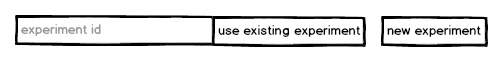
\includegraphics[width=1\textwidth]{web_id_uploadFields.png}
\caption{\label{fig:web_id_uploadFields}Fields for experiment selection/creation.}
\end{figure}

The upload view has two states, first the user have to choose if it wants to create a new experiment to upload files or use an existing file. This step looks like \refer{fig:web_id_uploadFelds}.

\begin{figure}[h]
\centering
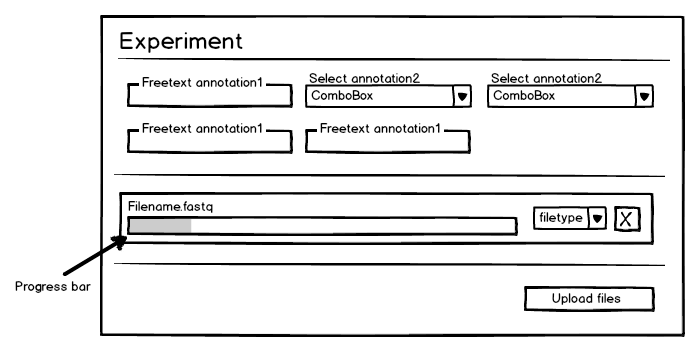
\includegraphics[width=1\textwidth]{web_id_fileUpload.png}
\caption{\label{fig:web_id_fileUpload}File upload and experiment annotation view.}
\end{figure}

Once the user has an experiment to upload files to it may start to upload files and annotate the experiment. The step for doing that looks like \refer{fig:web_id_fileUpload}.

\subsubsection{Process view}
The process view has a set of input and select fields for the user to input parameters to be used in the file processing. At the bottom of the view there’s a button used to start the processing.

\subsection{Systemadministration - Web}
The admin page is built up by four views: the navigation bar, the main view, the create annotation view and the edit annotation view. The first one is main view which consists of a navigation bar and a empty div-tag. 
The empty div-tag is then replaced with the annotation list view which has a Create new annotation button 
and a list of the available annotations on the database with an option to edit. 

When the user clicks on for example Create New Annotation, the div tag in the main view is replaced with the create annotation view.
The same goes for the Edit buttons on each annotation. This way we only have to render that specific div-tags current information 
and the navigation bar remains. 

The design is made so that the user should be able to avoid mistakes. For example in the 
create annotation page the user is not able to create an annotation without filling in all the fields. Futher more the 
field for Items in drop-down list is disabled if the user don't choose Drop-down list as the annotation type. 

In the Edit annotation view the same principles apply, but also there is a Delete Annotation button on this page which will
delete the entire annotation on the database. This made us ask two times if the user is sure of this action and ofcourse made the button red.

The back buttons on the different views work as any one using the internet is used to and the menubar option Annotations takes the user back to the main adminview.
\FloatBarrier
\section{Mobile clients}

\FloatBarrier
\subsection{Android}
The design of the android application is based on the design proposal suggested by the design team and our aim has been to recreate that look and feel. We did, however, find it necessary to take into consideration some of the android specific design paradigms which distinguish android applications from other smart phone platforms. For instance, the design put forth by the design group did not include a so called action bar   to the upper part of the user interface which are used for navigation. However, since these are fundamental to the structure of any android application, we were inclined to include this feature as a substitute for the slide-in menu described in the original design.

In the following sub-sections, we will compare the current design of our Android application (figures on the left) with the design proposal suggested by the design team (figures on the right), as well as attempt to explain our design desisions.


\subsection{Login View}
The two designs illustrated in figure \ref{fig:and_login} below are very similar except for the colour settings. There are textfields available for the user to type user name and password and a button to click when user is ready to log in. This is a popular layout for many login screens and thus a design many users are familiar with.


\begin{figure}[h]
\begin{center}


\begin{tabular}{c | c}
\addScaledImage{0.1}{andLogin.png} & \addScaledImage{0.47}{iosLogin.jpg} 
\end{tabular}
\caption{Android Login View vs iOS Design Proposal}
\end{center}
\label{fig:and_login}
\end{figure}


\subsection{Search View}
The two designs illustrated in figure \ref{fig:and_search} below are very similar. What is not depicted in the android view is the search button. It is, however, further down the item list and can be scrolled to.

\begin{figure}[h]
\begin{center}
\label{fig:and_search}

\begin{tabular}{c | c}
\addScaledImage{0.1}{andSearch.png} & \addScaledImage{0.47}{iosSearch.jpg} 
\end{tabular}
\caption{Android search view vs iOS design proposal}
\end{center}
\end{figure}


\subsection{Search Results View}
The two designs illustrated in figure \ref{fig:and_result} below are very similar except for the colour settings. The colour settings has changed since previous design since we adapted it to be more similar to the IOs design, which currently is designed using white background and black text. The list displaying search results is larger to facilitate usage for user and to take advantage of the screen space. It's easy to learn how to navigate the list. Scrolling is available if the list is long and if the user click on an experiment they are redirected to the experiment view displaying more information about that experiment.

\begin{figure}[h]
\label{fig:and_result}
\begin{center}
\begin{tabular}{c | c}
\addScaledImage{0.1}{andResult.png} & \addScaledImage{0.47}{iosResult.jpg} 
\end{tabular}
\caption{Android search result vs iOS design proposal}
\end{center}
\end{figure}

\subsection{Experiment View}
The two designs illustrated in figure \ref{fig:and_experiment} are similar except for colours and selection markers. The "slide bar" used for selection is not available in android and checkboxes has been used instead. All files for the experiment selected in the search result view is displayed here organised by data type. Checkboxes are commonly used and most users are familiar with how to handle them when making choices and selecting items. The button "Send to conversion" will be used to send selected files to the conversion view.

\begin{figure}[h]
\begin{center}
\label{fig:and_experiment}

\begin{tabular}{c | c}
\addScaledImage{0.1}{andExperiment.png} & \addScaledImage{0.47}{iosExperiment.jpg} 
\end{tabular}
\caption{Android experiment view vs iOS design proposal}
\end{center}
\end{figure}

\FloatBarrier
\subsection{iOS}

Focus has been on making a nice looking application with an intuitive workflow. The design is based on the design selected in the design phase. However, some changes has been made in order to follow the iOS design principles. New insights of the demands of the customer and our increasing experience has also resulted in improvements of the original design. Some of the design decisions are motivated in the text below.


\subsubsection{Navigation bar}
A navigation bar is used to make access to different main functionalities available at all times. The chosen design (at the end of the design phase) suggested to have an invisible menu which was slided in. However, an invisble menu is difficult to detect and does not follow the iOS design guidelines.


\subsubsection{Login Screen}
The login screen has two responsibilities; to make a nice first impression and to make it easy for the user to login. The design is kept simple and clean to avoid distractions.

\subsubsection{Search View}
The search view is designed to be usable for both advanced and new users. A list with available annotations is displayed to make it easy to do basic searches fast. Some annotations can only be selected with a picker view, while others are edited by typing free text. The reason for the occurance of the picker views is to simplify searches and help the user to make correct search requests. For example, the sex of an individual can only be male, female or unknown. Other values for the sex annotation would be nonsence!

\begin{figure}[ht]
\addScaledImage{0.2}{ios_search.png}
\caption{The search screen.}
\label{fig:ios_search2}
\end{figure}
\FloatBarrier

Each annotation has a corresponding switch button as seen in \refer{fig:ios_search2}. The button determines if the annotation should be included in the search request. This make it easy to make small changes to the search, while not clearing the annotation values.

The advanced user can customize the search query sent to the server. This gives the user the opportunity make more complex search queries and possibly make use of already accuried PubMed-search skills.

\subsubsection{Search Result View}
The main purpose of the search result view is to give an overview of the search results. The challenge with this view was to summarize large amount of information in a small area. The small screen of the iPhone made it impossible to have columns for each annotation. Instead a decision was made to group the files by experiment as seen in \refer{fig:ios_searchResult2}. The table with the experiments will only expand vertically, both when the number of shown annotations and the number of experiments grows. Thus, the user never has to scroll sideways which would be awkward.

\begin{figure}[ht]
\addScaledImage{0.2}{ios_searchResults.png}
\caption{The search result view.}
\label{fig:ios_searchResult2}
\end{figure}
\FloatBarrier

The user can choose which annotations to display in the result view. This gives the user the power to only show the annotations which are interesting at the moment. 

The file view (see \refer{fig:ios_files2}), which is shown when the user selects an experiment, only contains the most important information about the files of the specific experiment. The number of annotations shown in this view is kept at a minimun to avoid information overload and to give the user a good overview of the files. Three annotation were chosen: the name of the file, the date when the file was uploaded and the author. These were chosen to make it easy for the user to identify the correct files.

\begin{figure}[ht]
\addScaledImage{0.2}{ios_files.png}
\caption{The file view.}
\label{fig:ios_files2}
\end{figure}
\FloatBarrier

The functionality of the Convert files button can be reached from other views, but was added to this view as well to improve the workflow. Instead of first selecting the files, then going to the Selected files view and initiate the convertion from there, the user can now quickly convert files directly from the search results.


\paragraph{Selected Files}
The selected files view can be seen in \refer{fig:ios_selectedFiles2}. The files are grouped into four categories: raw, profile, region and other. This is done by showing each type of files in its own tab. The reason for this is to avoid the possibility to select files of different types since the tasks to perform are file type specific. It also gives a better overview of the files when only one type is shown instead of showing all files at the same time. Additionally, the top tab bar menu is following the iOS design guidelines.

\begin{figure}[ht]
\addScaledImage{0.2}{ios_selectedFiles.png}
\caption{The selected files view.}
\label{fig:ios_selectedFiles2}
\end{figure}
\FloatBarrier

\paragraph{Select task}
The select task menu can easily be expanded when new functionality is added to the application. The Execute-button is disabled as long as no task is selected. A checkmark is displayed next to the task to perform. When an other task is selected the checkmark is moved. The reason for not using switch buttons is that they would give the impression that several tasks could be executed at once, which is not possible at the moment.


\chapter{Architecture design}
%An overall look at how the architecture of the systems is designed. Communication diagrams and how the different parts interact with eachother. Directed towards developers.

To get an understanding on how the system is designed as a whole, this chapter will try to explain the architecture of the system on a more broad level.

% Here you can find a basic overview of the system in general.

\section{A system overview}

The \appName\ is a server-client system, which involves four different clients, a Java server and one postgresql database. The different kinds of clients are:

\begin{itemize}
\item iOS-client
\item Android-client
\item Web-client
\item Desktop-client
\end{itemize}


All of these clients use RESTful and Json to communicate with the server, sent over a non persistent HTTP-socket. How the different requests sent over this socket is specified in the API which can be found at : www........... 

Every request the client does creates a non persistent connection to the server. When the server receives a request it checks which kind of request it is and creates the corresponding internal command for it.

This command is an object which consists of information from the RESTful-header and Json body sent from the client. The command is sent to the database which returns information gotten by a SQL query. Depending on the requests this information can later be used to, for example processes a file or be sent back to the clients. The clients always going to receive a response code after each requests, but in some cases the respond also contains a Json body with information which can be shown to the user. This is the case for requests like getAnnotations.

After a client received the response the connections with the server disappears until the next request. 

There is a special kind of user called system admin. A user with these priveleges has the rights to add and delete annotations.

\begin{figure}[t]
\addImage{com_overviewImage.jpg}
\caption{A simple flow of data for the system}
\label{fig:com_systemOverview}
\end{figure}





\chapter{System design}
%A more indepth look at how the system is designed with UML- and class-diagrams. Directed towards developers. Start with subsubsection here.

A more indepth look at how the system is designed with UML- and class-diagrams. It is divided into two main sections for the server and clients. The client section contains the different clients. After that follows the server section that is divided into different parts that makes up the whole server. 

\section{Clients}
Here is an explanation of the  different client system designes.
\subsection{Desktop}
\subsubsection{Overview of the desktop client}
The \term{UML} diagram in \refer{fig:des_uml-overview} describes the whole desktop client.
\begin{figure}[htb!]
%	\addScaledImageVertical{0.172}{des_UML.jpeg}
	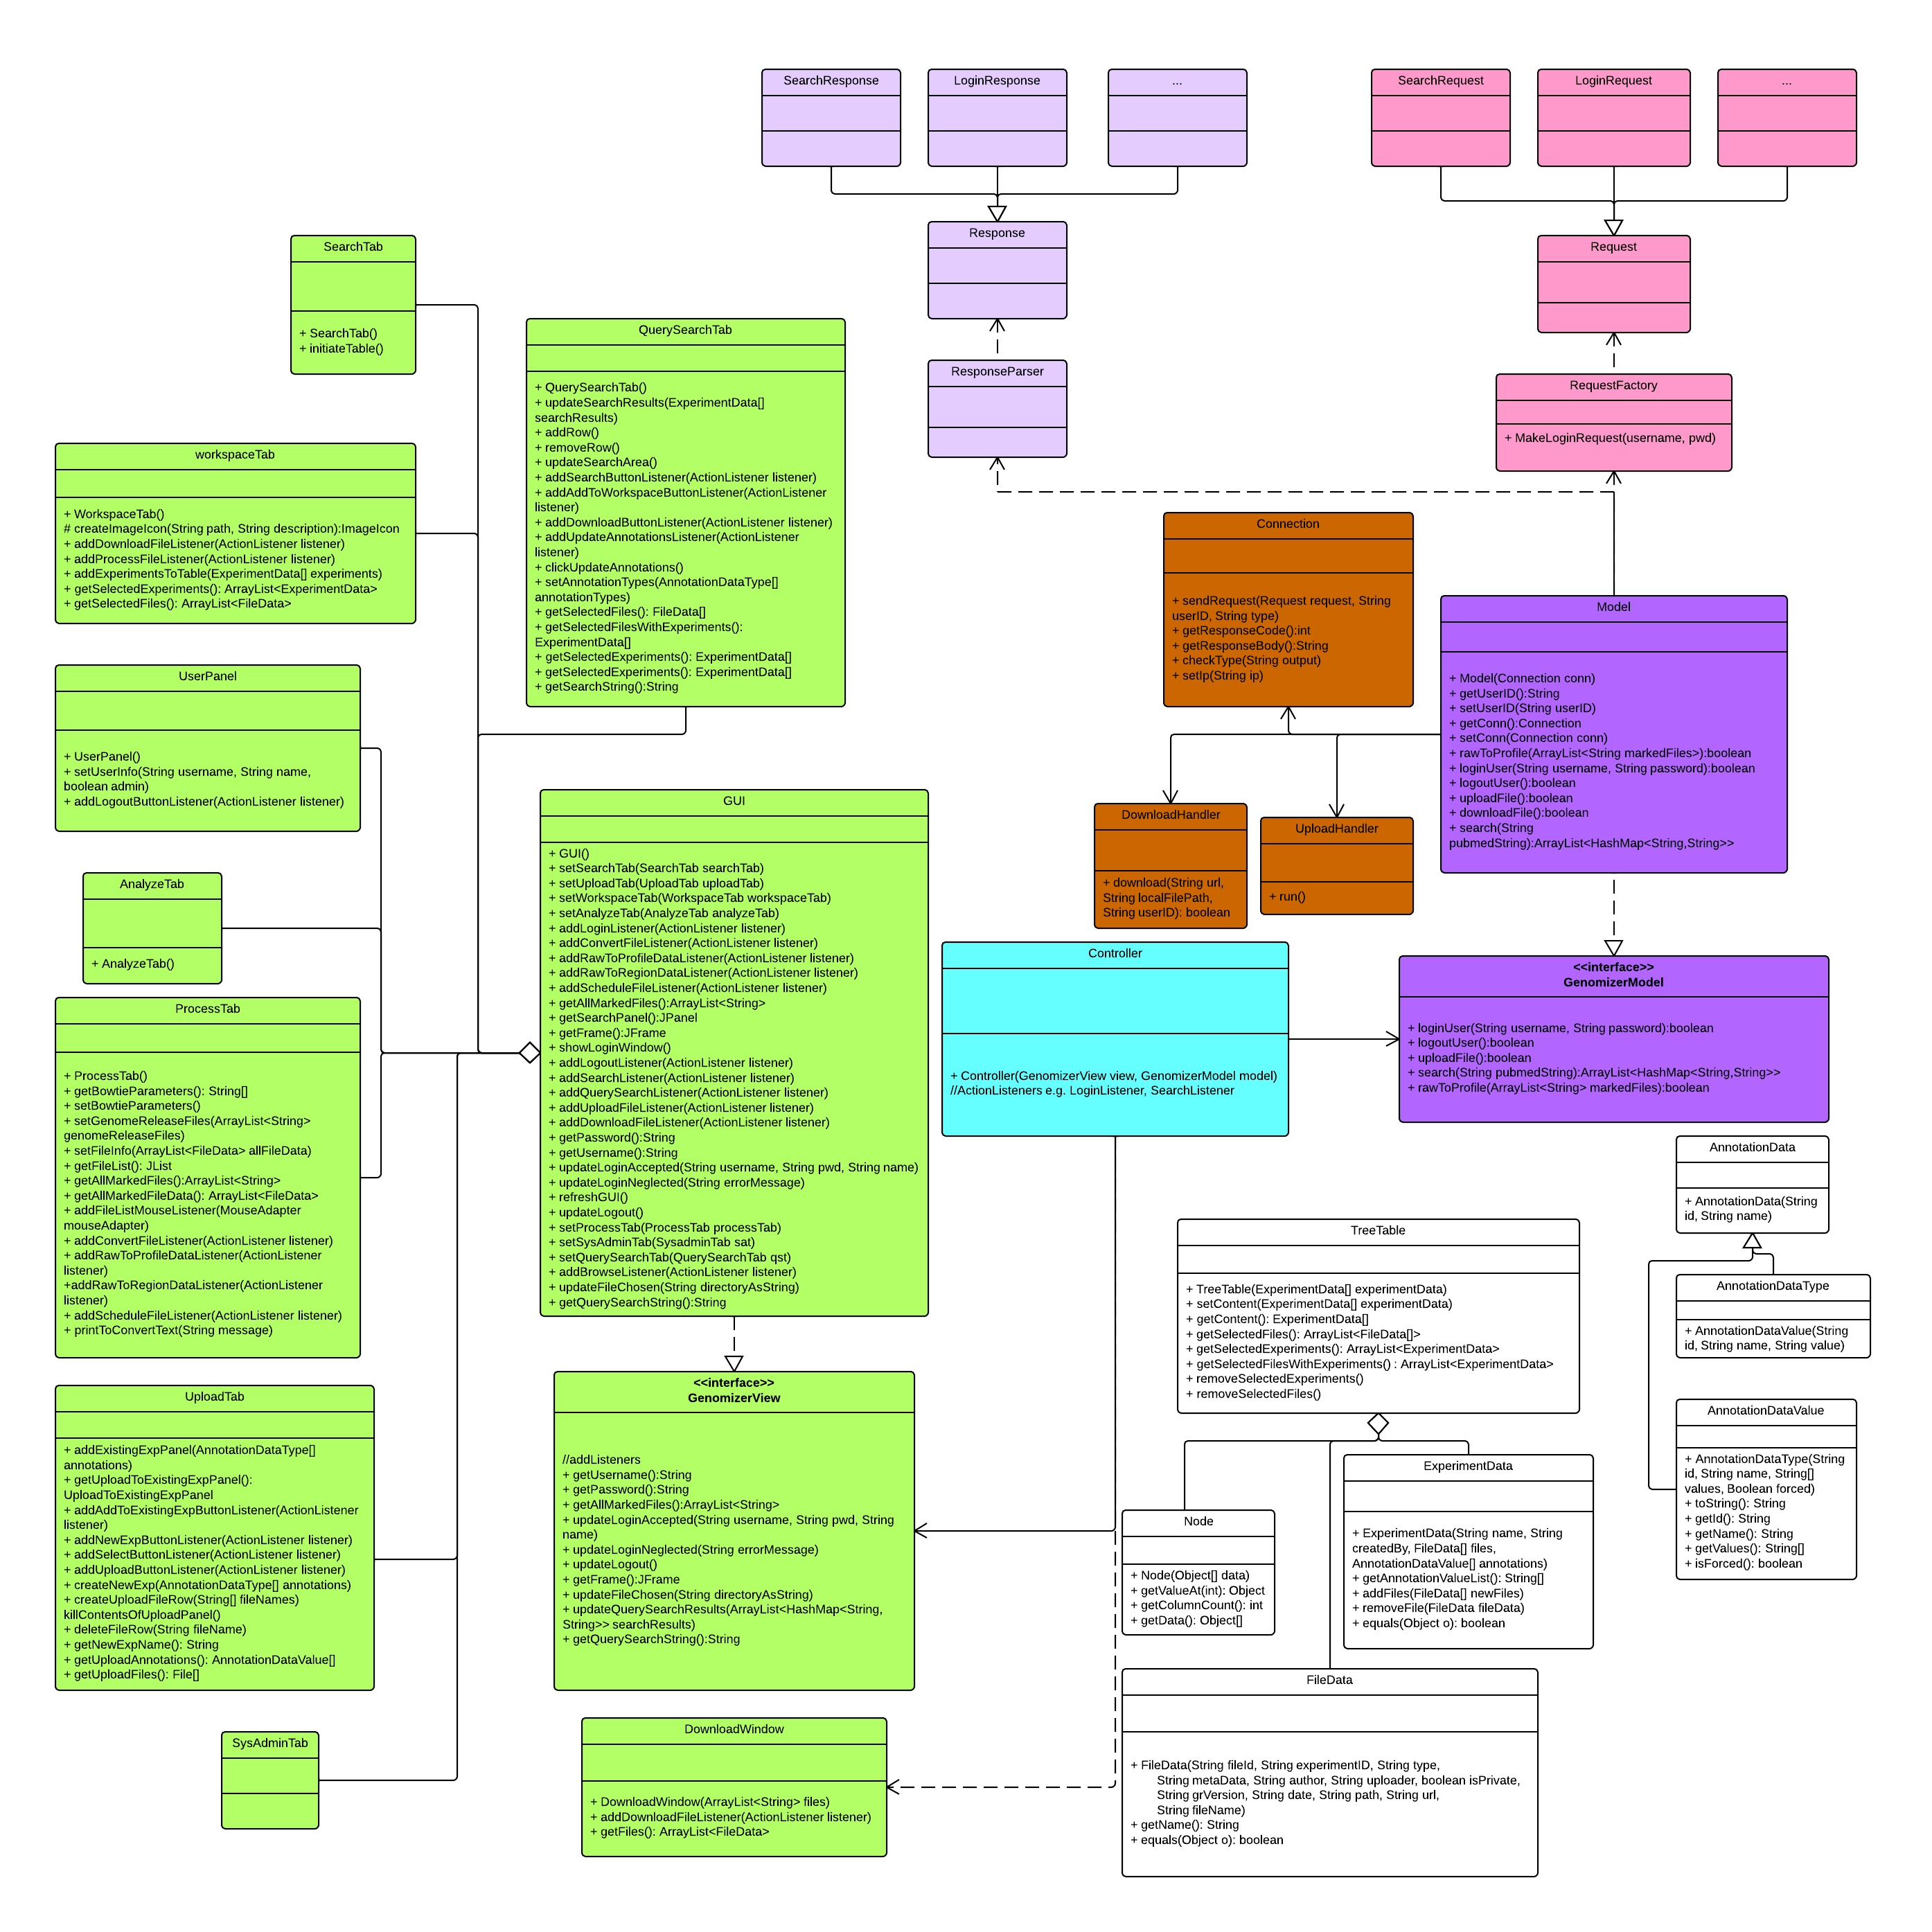
\includegraphics[width=\textheight,height=\textwidth, angle=90]{des_UML.jpeg}
	\caption{UML diagram over the desktop client}
	\label{fig:des_uml-overview}
\end{figure}

\subsubsection{View}
The view of the \appName\ Desktop client is constructed around tabs. There are 6 different tabs. These are \term{Search}, \term{Process}, \term{Upload}, \term{Workspace}, \term{Analyse} and \term{Administration}. In this version the \term{Analyze} tab is not used.

Each tab in the view is represented by its own java class. The \term{QuerySearchTab} class which represents the search tab can display both a search view and a results view. It uses the \term{QueryBuilderRow} class to construct the rows in the query builder which is used to construct search queries. The \term{QueryBuilderRow} class represents a row in the query builder and each row is dynamic and can change accordingly to user interaction.

The \term{UploadTab Class} represents the upload view of the \term{GUI}. It has functionality to both upload a file to an existing experiment (which is separately handled in the UploadExistingExpPanel) and to create a new experiment to upload files to.

The \term{ProcessTab} class represents the process view in the \term{GUI}. It contains a list where files to be processed can be stored and buttons and eight parameters for initiating the processing.

The \term{WorkspaceTab} class consists of six buttons and a \term{TreeTable} that holds all the experiments and their data. The buttons are: Delete from database, Remove selected, Download selected, Analyze selected, Browse local files and Process selected. From the workspace, the download function/window is accessible. The \term{DownloadWindow} holds the \term{FileData} to be downloaded and its \term{GUI} consists of a \term{JTable} showing the file names and has JComboBoxes for choosing file format and a download button which opens a JFileChooser to download files.

The \term{AnalyzeTab} Class is not yet implemented.

\subsubsection{Model}
The model part of the system contains method for doing most of the logic in the system. For example there are methods for sending login requests and for downloading files. There are separate classes for downloading and uploading files as well as a class for regular communication with the server called \term{Connection}.

\subsubsection{Requests}
The \term{Request} package contains the \term{Request} class , the \term{RequestFactory} and all the classes that extends the \term{Request} class. \term{Request} is the super class and can make a \term{JSON} package that all the other \term{Request} classes can use. All requests must have a name, type and an \term{URL}, but can consist of more information. For example \term{LoginRequest} also has username and password. \term{RequestFactory} is a class that can create all objects from all types of requests. It is a way to easily create all requests from the same place.


\subsubsection{Response}
This package consists of all types of responses that the server can send to the client-program. There is a class named \term{Response} that all the other response classes extends from. For example there is \term{LoginResponse}, \term{SearchResponse}. All these types of responses has different properties. There is also a class \term{ResponseParser} that can parse the responses so that the important information can be taken out of a \term{JSON}-package. This information can then be used to tell the client program what should happen next in the user interface. 


\subsubsection{Controller}
The controller part of the system consists of \term{ActionListeners} for the different buttons and functionalities in the view. For example there are Listeners for searching, downloading and processing. The Controller class has access to both the view and the model and acts as a middle hand between those two parts of the system. Usually a Listener in the controller reacts upon user input and then modifies the model and gives information about the change to the view.
\FloatBarrier

\subsubsection{Utilites}

There are several classes which represents different data in the system. There are classes for experiment data, file data and annotation data. For example when a search response is received from the server it is parsed into experiment data and the experiment data contains file data and annotation data.

The TreeTable class represents the table which displays experiment data, annotation data and file data in the Search and Workspace tabs. It is specially constructed to handle the data classes and it allows vertical sorting.

\subsubsection{System Administration}
%Till Anna!
The System Administration Tab is developed separeately from the rest of the Desktop GUI, and hence has it's own back end description here. 

\paragraph{Observer observable}
\label{Observer observable}

\begin{figure}[htb!]
\addImage{des_sysadminUML.png}
\caption{Communication UML}
\label{fig:adm_viewmodelcomuml}
\end{figure}

Observer is an interface and Observer is a class, and together they are used to simplify communication. This pattern is used when one object needs to be automatically notified of changes in another object. The observing object has to implement the Observer interface. This interface enforces only the \textit{update()} method which will be triggered every time something changes in the observed object. The Observable on the other hand is a class and any object that wants to be observed has to extend the Observable class. The Observable class has a few methods that can be of use but most important ones are \textit{addObserver()}, which is used to add an observer that will observe this object, \textit{setChanged()} simply sets flag that verifies that this object has changed, and finally \textit{notifyObservers()} that notifies all objects observing this object that something has changed and so triggers their \textit{update()} methods.

This pattern is used for communications between the system administration view and the main controller.

\paragraph{View to controller communication}


When the user requests a state change on the server of any kind, the following steps occur. When the user clicks the button to trigger the request a listener will fetch the data from the GUI and package it into a specific datatype. When finished the listener triggers the \textit{notifyObservers(<object>)} method with the datatype as an argument. Which in turn triggers the \textit{update()} method in the \textit{SendDataObserver} class located in the main controller. The \textit{SendDataObserver} unpacks the data and then calls the model which creates the request.

In \refer{fig:adm_viewmodelcomuml} an example of this communication flow is visible. An example is when a user wants to create a new annotation. Once the user has filled in all the neccesary fields in the new annotations view, the user clicks the 'Create annotation' button (See \refer{fig:adm_desktopgui}). The \textit{AnnotationPopupListener} receives the event and calls the \textit{sendNewAnnotation()} method in the \textit{SysadminController} class. This method then creates an instance of the datatype \textit{AddAnnotationRequest} using the input from the textfields in the \textit{SysadminAnnotationPopup}. Since the  \textit{SysadminController} is an Observable object, it then uses the inherited methods \textit{setChanged()} and \textit{notifyObservers()}. This triggers the \textit{update()} method in the \textit{SendDataObserver} class (which implements the Observer interface and is an inner class of the \textit{Controller} ). The \textit{update()} method only receives an object, so first it verifies that the Object is of the \textit{AddAnnotationsRequest} type, and then extracts the neccesary attributes from the datatype and sends them to the \textit{GenomizerModel} which create the request.





\subsubsection{Annotation}

The annotation tab is implemented in the class \textit{AnnotationsViewCreator} 

\paragraph{Add annotations}
When adding a new annotation which is done from the popup window that is implemented in the \textit{SysadminAnnotationPopup} class, the \textit{AnnotationPopupListener} recives an event. The event is parsed and the \textit{sendNewAnnotation()} method will be executed in the \textit{SysadminController} class. Here the input from the user will be fetched and sent into a new datatype object of \textit{AddAnnotationRequest} (located in the \textit{requests} packet). This object will in turn be sent to the model via the observer observable (see \ref{Observer observable} - Observer observable) design pattern that is implemented. 



\subsubsection{Flow of the system}

The sequence diagram in \refer{fig:des_download-sequence} describes the flow of the system when the user presses the download file button and the diagram in \refer{fig:des_login-sequence} describes how the desktop clients reacts to a login.





\begin{figure}[htb!]
	\addImage{des_downloadsequence.jpeg}
	\caption{UML sequence diagram of downloading a file}
	\label{fig:des_download-sequence}
\end{figure}

\begin{figure}[htb!]
	\addImage{des_loginsequence.jpeg}
	\caption{UML sequence diagram of login}
	\label{fig:des_login-sequence}
\end{figure}
\FloatBarrier

\FloatBarrier
\subsection{Web}
This section describes the design of our system, first with a system overview and then with more indebth information about our tabs.

\subsubsection{How our web application works}
%figure x5
\begin{figure}[ht]
\centering
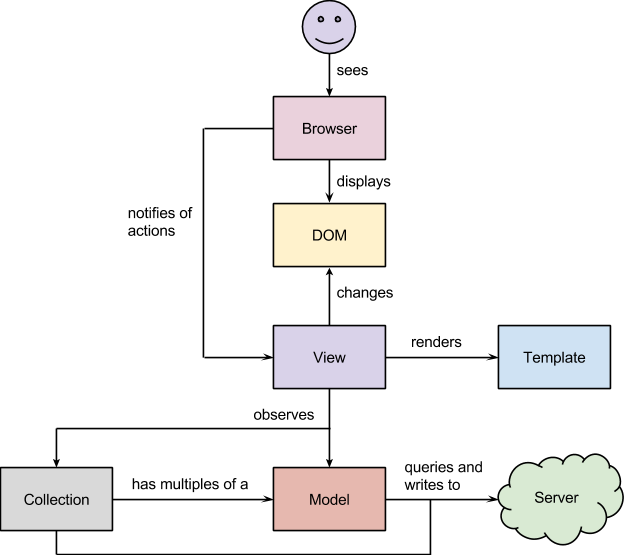
\includegraphics[width=1\textwidth]{web_system_backboneWebapp.png}
\caption{\label{fig:web_system_backboneWebapp}A general build of a backbone webapp.}
\end{figure}

\refer{fig:web_system_backboneWebapp} shows how a backbone\cite{web_1} web application works in general. We have a user, that interacts with a browser. A browser renders the DOM of our web application. How it does this is up to the browser. Different browsers might display it differently. Models and Collections will talk to the server to update themselves. For example, our \textit{Experiments} collection will retrieve experiments from the server and update itself with a call to it’s fetch() method. Out of the components that go into this figure, we are in charge of and only capable of changing a few of these; \textbf{View}, \textbf{Template}, \textbf{Collection} and \textbf{Model}. See the Backbone section of Frameworks in section \ref{sec:web_frame} more information.

\subsubsection{System overview}
%figure 2
\begin{figure}[ht]
\centering
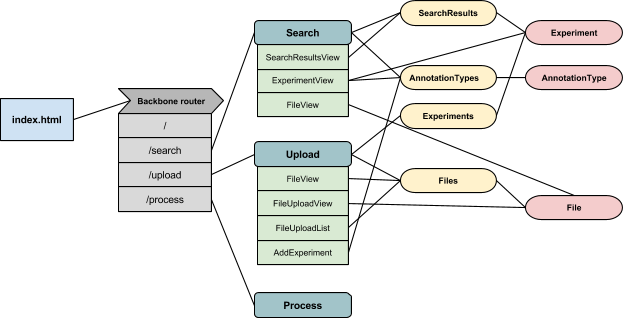
\includegraphics[width=1\textwidth]{web_system_overview.png}
\caption{\label{fig:web_system_overview}Overview of the relations between the different javaScript prototypes in the system.}
\end{figure}

Since our app is built using Backbone\cite{web_1}, our app is divided into the parts \textbf{Misc}, \textbf{Views}, \textbf{Collections} and \textbf{Models}. In \refer{fig:web_system_overview}, we can see the system overview. The \textbf{views} are the parts in green, the \textbf{collections} the parts in yellow and the \textbf{model} the parts in red. The parts in grey represent the router which belongs in our Misc category. It is responsible for rerouting links. For example, when a user clicks the search tab, the router navigates to /search, but instead of loading the whole /search over the page we are currently on, our router will open our search tab below our navigation bar. The \textbf{Misc} category also holds our Main.js, which is in charge of setting up and starting the app.

\subsubsection{Search}
The search tab has three views, the main one being \textit{Search}, which acts as a container for the \textit{SearchResultsView}and holds the search input field and the various buttons displayed. The \textit{SearchResultsView} handles rendering the annotations and the \textit{ExperimentViews}, where one \textit{ExperimentView} is created for every experiment returned from a search. The actual data retrieved is stored, by experiment, in \textit{Experiment models}. To organise this data, we have a collection to contain all the experiments retrieved, called \textit{SearchResults}.
 
%figure bla bla/lalalallala
\begin{figure}[ht]
\centering
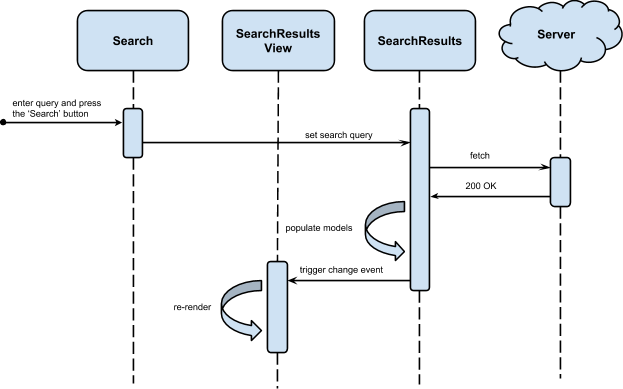
\includegraphics[width=1\textwidth]{web_system_sequenceDiagram.png}
\caption{\label{fig:web_system_sequenceDiagram}a sequence diagram showing what happens when a user enters a valid search query and results are fetched.}
\end{figure}

In \refer{fig:web_system_sequenceDiagram} is a simple sequence diagram for the search tab. If a user enters a query in the search field and then presses the search button, the \textit{Search} view will update the \textit{SearchResults} collection to have a new query. Once \textit{SearchResults} has a new query, it will try to fetch search results corresponding to the query from the server. If successful, new experiment models for every experiment retrieved will be created and set in the \textit{SearchResults} collection. \textit{SearchResults} then triggers a ‘change’ event that \textit{SearchResultsView} listens to. When that event occurs, \textit{SearchResultsView} knows that \textit{SearchResults} has been changed, and re-renders itself.


\subsubsection{Upload}
The upload tab has three main views, the main one being Upload, which acts as a container for the ExperimentView’s and holds the search input field and the various buttons displayed. Each ExperimentView handles rendering the AnnotationsForm and the FileUploadList, where one ExperimentView is created for every experiment the user inputs. The actual annotation data and files input by the user is stored, by experiment, in Experiment models. To organize this data, we have a collection to contain all the experiments input, called Experiments.
\subsubsection{Process}
To be announced.
\FloatBarrier
\subsection{Android}
This section describes the architectural design of the Android application. All coded functionality is described in this section, inluding the functionality that is not fully integrated. 
\subsubsection{Class descriptions}\label{sec:and_classdescription}
This section focuses on the functionality of each class.

The connection between the classes labeled model can be seen in \refer{fig:and_umlmodel} while the other classes can be seen in \refer{fig:and_uml}
	\begin{figure}[h]
		\addImage{and_UML_model_sprint2.jpg}
		\caption{Android UML of model}
		\label{fig:and_umlmodel}
	\end{figure}  
\begin{figure}[h]	\addImageVertical{and_UML_android_sprint2.jpg}
		\caption{Android UML without model}
		\label{fig:and_uml}
	\end{figure}  
    \FloatBarrier
\subsubsection{Android activities} 
Activities are used as frames to display various fragments. For anything to be displayed it must be a part of a fragment that is a part of an activity. Each activity used in this application extends the class SingleFragmentActivity which has the purpose of creating a new fragment of an arbitrary type that displays a single fragment. This means that in its current state the application contains one fragment per activity and each fragment described in this section is coupled with an activity
\subsubsection{Fragment Class: LoginFragment}
This fragment will be the first view the user sees when the application is started, it allows the user to specify username and password. ComHandler \ref{sec:and_class_comhandler} is then used to send and validate the login request. If the username and password are incorrect the user will be informed through an android toast explaining what happened. Likewise if the server cannot be reached.

A successful login will start the SearchListFragment \ref{sec:and_class_search}.
\subsubsection{Fragment Class: SearchListFragment}\label{sec:and_class_search}
Handles the search-view for the \appName\ app, the annotations that can be chosen are downloaded from the server and they are, as such, dynamic.
\subsubsection{Fragment Class: ExperimentListFragment}
This fragment handles the displaying of search results to the user. The fragment includes a ListView with an ArrayAdapter set to it. An OnItemClickListener is used to detect when the user is selecting an item in the list and is currently starting FileListActivity \ref{sec:and_class_filelist} when a list item is selected. This fragment receives a HashMap with search values from SearchListFragment \ref{sec:and_class_search} and when activity is starting an ASyncTask is started to send and receive search results from the server through the ComHandler \ref{sec:and_class_comhandler} class. When an experiment is selected from the list the file names belonging to that experiment is sent to FileListFragment \ref{sec:and_class_filelist} that will display the file information. 
\subsubsection{Fragment Class: FileListFragment}\label{sec:and_class_filelist}
This fragment displays all files associated with a chosen experiment. The fragment is using three ListViews, one for each data type. The data types that are available are: raw, region and profile. Each list element will show the name of the data file and have a checkbox connected to it. A custom ArrayAdapter is used to handle checkbox interaction and displaying information to the user. There is option to select multiple files in the view by checking several checkboxes. The file names displayed are the ones currently available from the server for each available experiment.
\subsubsection{Model Class: ComHandler}\label{sec:and_class_comhandler}
Is a static object that is called by the fragments in the view to gain access to the models different functions. At this stage the ComHandler can be used to login, search for files and to request raw to profile conversions, although the latter is not yet integrated. The url that ComHandler tries to communicate with can be changed with a public method which makes it possible to implement a way for the user to change server.
\subsubsection{Model Class: Communicator}
Intended to manage the sending and receiving of messages between the server and the application using a http connection.
\subsubsection{Model Class: MsgFactory}
Creates the JSON messages that can be sent to the server.
\subsubsection{Model Class: MessageDeconstructor}
Interprets JSON messages and returns appropriate information.
\subsubsection{Model Class: GenomizerHttpPackage}
Used to store the body and status code of an http-response.
\subsubsection{Model Class: GeneFile}
Used to store and transfer the information of a genome file.
\subsubsection{Model Class: Annotation}
Used to store and transfer one or several annotations and their value.
\subsubsection{Model Class: Experiment}
Used to store and transfer information about an experiment.
\subsubsection{Model Class: ProcessingParameters}
Used to simplify the transfer of parameters in a processing request.

\FloatBarrier
\subsection{iOS}
System design for the Genomizer iOS application. The  system is designed using the model-view-controller principle. Each view is controlled by its own controller class.
\begin{figure}[ht]
\addScaledImageVertical{0.3}{ios_UML.png}
\caption{UML diagram .}
\label{fig:ios_UML}
\end{figure}

\refer{fig:ios_UML} gives an overall image of the system design. Some classes are excluded from the figure due to making it easier to get an overall idea of the system. The controller classes of the table cells and some other controller classes are not illustrated in the diagram. The non-excluded are explained below:

\FloatBarrier
\subsubsection{DataFileViewController}
Controlls the File view presented in \refer{fig:ios_files}. It contains a referens to an experiment and lists all its files in a table.

\subsubsection{SearchResultController}
Controller class for the Search Results view presented in  \refer{fig:ios_searchResult}. It configures the table which holds the information about the experiments a search resulted in. An ExperimentDescriber is used to generate a description of the experiments.

\subsubsection{ExperimentDescriber}
Generates a description of an experiment using annotations chosen by the user.

\subsubsection{Experiment}
A class that contains all information related to an experiment.

\subsubsection{ExperimentFile}
Is a class that contains information about a file from an experiment.

\subsubsection{ExperimentParser}
A class that parses experiment information from a NSDictionary to an Experiment object.

\subsubsection{SearchViewController}
Controller class for the Search view, see \refer{fig:ios_search}. It checks which annotation-fields are used and tells the JSONBuilder to generate a corresponding search query when the user presses the search button. The class also contains a advanced search to allow the user to manually enter search queries. 

\subsubsection{Connection}
A class that sends and receives JSON objects to and from the server.

\subsubsection{JSONBuilder}
A class that can create diffrent JSON requests.

\subsubsection{Selected files}
The selected files controlls the selected files view shown in \refer{fig:ios_selectedFiles}. The selected files class contains information about files saved by the user. It has a method that can make convertion possible. 

\FloatBarrier
\section{Server}
The system design of the different parts of the server.
\subsection{Communication}
The server system is based around HTTP, where clients send requests on a non-persistent connection and the server responds to these requests. All communication is initiated by the client and the server has no way of contacting clients except when responding to a request. 

Clients send requests to the communication part of the server first. When a request is picked up by the server, the request is parsed and a command is created depending on the request. The command then communicates with the other parts of the server in order to get or input relevant data. 

To identify clients a unique token is used, which is generated when a user logs in. The token is sent back to the client, and the client must include this token with all following requests. Since there is no persistent connection between the client and the server this token is the only way for the server to identify the sender of any given request. The token is also used to prevent unauthorized requests from being executed on the server.

Most commands are executed immediately when the server gets a request, and the result is sent back to the client when the command is finished. This happens when for example searching the database. 

The commands implemented for the server are:

\begin{itemize}
	\item $login$
	\item $search$
	\item $annotation$
	\item $experiment$
	\item $file$
	\item $process$
\end{itemize}

The $login$ command can take either a $'POST'$ method or $'DELETE'$ method, depending on if the user wants to log in or log out. 

$Search$ is used for searching for experiments in the database. Results will display all experiments which match the search query, and the user can chose o expand these experiments in order to view the containing files. 

The $annotation$ command can be used to modify and view annotations associated with experiments. The server can respond to a $'GET'$ request with an array of all possible annotations currently in use in the database. There is also possible to add new annotations, update the values for an annotation or delete a complete annotation field. 

Clients can get information about a specific $experiment$ by using a $'GET'$ together with this command. The server will respond with information about the experiment aswell as information about all the files associated with the experiment. Clients can also add, modify and delete experiments. 

An experiment contains $file$s which can be uploaded with this command. A $'POST'$ will let the client upload a file to a specific experiment. Clients can also download, modify and delete files. When a client downloads a file, the communication part of the server is never contacted. This is because a download URL is already present in the file on the client side. Therefore no contact is needed with the communication part of the server, but instead the file system server takes care of the request. 

In order to convert files, the client can send the command $process$. This will convert specific raw files into profile files.
\FloatBarrier
\subsection{Conversion}
The Genomizer service needs to be able to convert, process and visualize data. This chapter explains how this is done in the system.

\begin{figure}[h]
\addImage{con_UMLsprint2.jpeg}
\caption{Classdiagram for Process}
\label{con_UML}
\end{figure}
	
As can be seen in \refer{con_UML} the RawToProfileConverter extends the Executor class. When a call comes to the ProcessHandler it then starts the correct convertion which right now only can be a raw to profile convertion.


\subsubsection{Executor}
The executor class, as seen in figure 5.2.1, is an abstract superclass that is an entity that is able to execute various commands. The executor class is able to run programs as well as scripts. In order to run scripts and programs the executor has a parse-function that parses a string into separate arguments. \newline

\begin{itemize} 
\item executeCommand
\begin{itemize}
\item ExecuteCommand is a private method that is being used by the executeScript, executeProgram and executeShellCommand methods. Firstly a processBuilder is used to ensure a safe way to execute commands, after that the working directory is set and the error output stream is merged with the standard output.
After a command has been started the output stream is then recorded with the help of a scanner object and a stringBuilder object. When the command has been executed the recorded string is sent back to the caller.
\end{itemize}
\item executeScript/executeProgram
\begin{itemize}
\item Both methods are very similar. The difference is that executeScript has a static filepath added to the second argument. This is because the first argument when calling a script is the script language instead of the actual script file. E.g. shell resources/script.sh.
\end{itemize}

\item parse
\begin{itemize}
\item In order to receive a command string and to be able to run it a parse method had to be implemented. This is because the processbuilder takes a String array as argument. With the help of a tool called stringTokenizer the string is parsed into a String array separated on spaces.
\end{itemize}
 
\item cleanUp
\begin{itemize}
\item Deletes a folder and all its contents, it takes a File object and recursively removes everything in that folder and its subfolders. Used to clean up files created when doing a procedure that creates temporary files thats not used after the procedure is done.
\end{itemize}

\end{itemize}

\subsubsection{RawToProfileConverter}
\emph{The purpose of the RawToProfileConverter class is that it will be used by processHandler and do all the different steps needed to make a raw file. These steps are done by using the program Bowtie and by running four different scripts which are executed with methods that is extended from Executor class. When ratio calculation is supposed to be done, there are two more steps that will be done.}

\begin{itemize} 
\item procedure
\begin{itemize}
\item This method executes all the methods for all the steps to make a profile .sgr file from a raw file, it checks so that the directory it gets that should contain the raw files has not more then two files and atleast one file to process. Does the procedure to create a profile data and move it to the folder thats specified as a parameter.
\end{itemize}

\item runBowtie
\begin{itemize}
\item Constructs a long string with the full execution line for bowtie. It then uses this string as a parameter when calling the method parse. 
The resulting array is then using when calling executeProgram and the result of the execution is returned.
\end{itemize}
\item sortSamFile
\begin{itemize}
\item Constructs a string with the full execution line to sort a sam file. It then calls parse to create a string array from the full string and sends it as parameter to executeShellCommand which runs a shell command to sort the file and creates a new .sam file that is sorted with the specified parameters.
\item makeConversionDirectories
\begin{itemize}
\item Creates the necessary directories used by RawToProfile's procedure to put the temporary files needed to do all the steps to create a profile .sgr file.
\end{itemize}
\item initiateConversionStrings
\begin{itemize}
\item Defines all strings needed for the directories created when procedure is doing its work. Also defines a string for each step in the procedure, which gets passed to the corresponding execute methods. 
\end{itemize}
\end{itemize}
\end{itemize}

\paragraph{Bowtie}
Bowtie takes two raw .fastq files and converts them to .sam which is the first step to make the desired .sgr files. After a .sam file is converted the linux command sort is run  on both files which creates two sorted .sam files, it is sorted by chromosome and position as needed to use the scripts.

\paragraph{Used scripts}
The different functions of the perl scripts is explained below. They are explained in the same order that they are executed. All scripts take a directory of files to be processed as input parameter.


\subparagraph*{samtoreadgffv1} Makes a .gff file from a sorted .sam that have reads at each nucleotide positions. No input parameters except the directory of the sorted sam files are needed. The resulting files are put in the new folder \term{reads\_gff}.

\subparagraph*{readsgfftoallnucsgrv1}  Counts the reads from the previous script result. For each chromosome reads are read and each nucleotide position is incrementally counted with one when a read cover it. No parameters are needed for this script except the file path of the gff files. The resulting files are put in the new folder \term{allnucs\_sgr}.

\subparagraph*{smoothv4} Smoothing is done by using a script with the same name and it can smooth the single nucleotide reads with different options like short window sizes, what kind of smoothing is desired, minimum step position and the choice to choose if the result file should contain median values and/or 0’s. An example of input parameters to this script is: "10 1 5 0 0". The resulting files are put in the new folder \term{smoothed}.

\subparagraph*{AllSeqRegSGRtoPositionSGRv1}  converts the previous result in .sgr format to an .sgr format with fixed interval size. The script takes two parameters, if steps should be created and the stepsize. An example of parameters to the script would be: "y 10". The resulting files are put in the new folder \term{Step10}.



\subsubsection{ProcessHandler}
The processhandler is a controller that handles process-calls. Depending on the name of the process it handles it differently. It acts as an interface between the process-module and the rest of the program. 


\subsubsection{Logic \& interface}
The main logic in the processHandler is a switch-case that switches on the name of the process being called. For example if the name of the process is “RawToProfile” is sets up a RawToProfile-converter and calls it. 

\subparagraph*{processName} A string that tells the handler which kind of process should be executed.
\subparagraph*{procedureParams} A list of string with the parameters to the different external  programs/scripts that will be called during the execution. The first element will be a string with parameters/flags for the first external program that will be called, and so on.
\subparagraph*{inFile} A string with a path to the directory containing the files that should be operated on.
\subparagraph*{outFile} A string with a path to the directory where the result .sgr files should be put.





\FloatBarrier
\subsection{Filetransfer}
In the current version of the program the desktop clients and the web clients connect to different software on the server for communication. The desktop clients connect directly to the server communication software whilst the web clients connect via the apache server and all non web requests that is to be calculated using the server software is automatically redirected by apache.
The redirect is setup in a way that all GET requests that have a /api/ tag in the url will be redirected.
The exception for the desktop clients are file up- and downloads which are done through the apache server.

The download and upload will work for all platforms although this will not be implemented for Android and iOS clients due to hardware limitations.

If the client wishes to upload a file to the server they first send a request to the server-system which authenticates the client and stores the annotations for the file. Since the authentication is handled by the server software the path to where upload is done is not checked in this stage of the development.

For uploading and downloading files via Apache, two php-scripts will be used. If the user wants to upload a file, the php-script will try to store the file in a location on the server provided by the client. If this fails a ‘406 Not Acceptable’ status code will be returned. A script for downloading files from the GEO database and saving them on the server is currently being  implemented, although not yet fully tested nor implemented by the clients. See \refer{chap:servercmd} for examples when using the php-scripts.

In \refer{fig:exp_flow} below it is shown how the systems handles the different types of messages the client-systems can send. The big square represents the Apache server with different parts of the Apache server within. The iOS and Android clients can only send some requests to some computation to the server-system. Meanwhile the desktop client can send requests to the server-system and upload and download to/from the web server. The web client sends all its messages to the Apache server and if it is a request to do some sort of computation it will be redirected to the server-system and if it is a download, upload or webpage message it will be sent to the web server.

\begin{figure}[hbt]
\addImage{exp_flow}
\caption{A figure showing the different types of messages sent between the systems.}
\label{fig:exp_flow}
\end{figure}

The current version of the system utilizes a file structure to organize html- and file requests on the server, the structure is illustrated in \refer{fig:exp_filestructure}. The Web-root folder houses the php-script for uploading and downloading files. The app folder contains the \appName\ web page. In the data folder are all the expirements folders, which contains folders for the different data-types.

\begin{figure}[hbt]
\addImage{exp_filestructure}
\caption{Figure illustrating the current file tree on the server machine.}
\label{fig:exp_filestructure}
\end{figure}
\FloatBarrier
\subsection{Database}
Our system for the file storage is basically built up with a database and a file system, where the header information of a file is stored in the database and the real file is stored in the filesystem. A filepath string is stored in the database as “path”, so the user can find where the actual file is stored in the filesystem. You can see the database design in the schema below (\refer{fig:dat_databaseSchema} ). \\

Note that this section only describes the advanced system design that needs further explanation than just reading the code. Also note that it exists some javadocumentation that explains all methods in each class further deeper and more specific than this documentation that might be useful for those that will continue developing this system. Those can be found in the same file directory as the program, in the sub dir "/doc".

\begin{figure}[htb]
\addImage{dat_schema_V3.jpg}
\caption{Schema for the database.}
\label{fig:dat_databaseSchema}
\end{figure}

\underline{Comments about the database design:}

* FileID is a unique number for a specific file. It will be autogenerated by the database when you insert one file row.\\
* Path is where the actual file is stored in the filesystem, example:

\centerline{$home/data/experiment_1/raw/rawFile1.raw$}

Since many files are stored in pairs, the InputFilePath is the path to where the other file pair  is stored.\\
* MetaData is the arguments used when converting. \\
* IsPrivate is a boolean (T or F) for making the file private or not.\\
* Role in User Info determines the user rights for one user in the system, examples could be admin, user, etc.\\
"Annotated With" is the table that connects one experiment to one annotation, example:
\begin{center}
  \begin{tabular}{| l | l | l | l|}
    \hline
    $Experiment_1$ & Species & Dog\\ \hline
  \end{tabular}
\end{center}
* "Annotation" is the table containing the annotation with a preset default value, but not any choices. example:
\begin{center}
  \begin{tabular}{| l | l | l | l|}
    \hline
    Species & DropDown & Human & T \\ \hline
  \end{tabular}
\end{center}
"Annotation choices" is the actual values for a specific annotation, example:\\
\begin{center}
  \begin{tabular}{| l | l | l | l|}
    \hline
    Species & Dog \\ \hline
    Species & Fly \\ \hline
  \end{tabular}
\end{center}

\subsubsection{Methods description}
Below is some interaction processes described and what happens in the \term{database\-Accessor} class that needs further description than just viewing the class or the javaDoc.\\
\\
\underline{GetExperiment:} Will find a specific experiment from one experimentID, from the database and will return an experiment object for that experiment. The object will contain information about the experiment id, experiment annotations connected to that experiment, and all files connected to that experiment with their headers. The object contains both setter and getter methods. \\
\\
\underline{Adding one experiment step by step:}
There are some steps that need to be done in the right order to be able to add one experiment into the database. The order is as follows:\\
\\
1: First you will need to call the "addExperiment" method. It will add one experiment to the database witout any annotations set to that experiment. 

2: Then you add the annotations in general that should exist in the database.This can be done in many different methods depending on what purpose the annotation should have. Those are:\\
\\
a) AddFreeTextAnnotation: adds a free text annotation that will not be visible as a dropdown choice for the gui. Example for one entry line in the database could be: "Tissue,FreeText,Null,T".\\
\\
b) AddDropDownAnnotation: adds one annotation that will be visible as a dropdown choice for the gui. This method wants the label and a list of all annotation choices that the label should have, and also a default value. This method will fail if that annotation already exists in the database. Example of one entry could be: "Sex, DropDown, Male, T".\\
\\
c) AddDropDownAnnotationValue: If the method above fail because that annotation already exist in the database, you can run this method to just add one annotation choice to one existing annotation label, example: "species,dog".\\
\\
3: Once the annotation is set, you can connect the experiment with the annotations. This is done by calling the method "annotateExperiment". It is also here the FreeText annotations stores its values.\\
\\
Now the experiment should be in the database with annotation values, and is now ready to have files added to it.\\
\\
\underline{Changes to Annotations:} The possible methods for changing existing annotations are:\\
\\
* ChangeAnnotationLabel: changes one entire label in the database.\\Example: "Sex, Tissue, etc.".\\
\\
* ChangeAnnotationValue: change one value for a specific annotation label.\\Example: "male,female,fly,etc.".\\
\\
* GetChoices: Gets you all the available annotation choices connected to one label that you send in as inparameter. Example is "sex" that might return a list with values "Male,Female,Unisex,Unknown".\\
\\
* GetAnnotations: returns all annotation labels currently stored in the database. Examples could be "Sex,Species,Tissue,etc.".\\
\\
* GetAllAnnotationObjects: Does the same as the method GetAnnotation, but return it as an arrayList instead.\\
\\
* GetAnnotationObject: one method where you send in one label and get back one annotation object containing the "annotation" row  from the database, aswell as all its connected annotation choices.\\
\\
* GetAnnotationObjects: Same as getAnnotationObject but it returns a list of annotation objects from a list of annotation labels.\\
\\
* DeleteAnnotation: Deletes an entire annotation from the database. Since the database is configured to delete on cascade, all annotation choices connected to that annotation label will be removed, also the connection to the experiments with that annotation label.\\
\\
* RemoveAnnotationValue: Removes a single annotation value connected to a label, for example: "fly", or "arm".\\
\newpage
\underline{Adding files:} To add a file you will need to have an experiment added before you call the "addNewFile" method. Some files uses multiple files like raw data so make sure that you upload them together and that the "InputFilePath" points to their other file pair.\\
\\
\underline{Removing files:} Also here, if you delete one file that comes as an file pair, you must also delete the other file thorugh this method.\\

\underline{Other:} There exist other methods as well, but these does not need any further description then what is written in the java class DataBaseAccessor. Down bellow follows a more overall description of each class that is needed in the datastorage part of the system.\\

\FloatBarrier
\subsection{Apache}
The Apache HTTP Server or commonly referred to as Apache, is the web server application that was decided to be used to upload and download files to and from the server. Apache is open source, that makes it free to use. Apache is a good choice because it is developed and maintained by an open community, that way all new versions and updates will become available for free. And since it is open source, the source code is open for everyone to read. Apache can be used on both Unix/Windows systems, but in this case it is currently running on a Unix machine but can still communicate with all platforms. 

\subsubsection{Server user manual}
The Apache server is controlled from the terminal, this can be done either directly from the server or remotely from another computer using ssh. To use ssh from another computer, write

\texttt{ssh pvt@scratchy.cs.umu.se -p 2222}

in the terminal, when asked for password enter the password for the server. Then write the commands directly in the terminal.

These are some of the most common commands for apache: \\
\begin{tabular} {| l | l |}
\hline
\textbf{Action} & \textbf{Command} \\
\hline
Start Apache & \texttt{sudo service apache2 start} \\
\hline
Stop Apache & \texttt{sudo service apache2 graceful-stop} \\
\hline
Restart Apache & \texttt{sudo service apache2 graceful} \\
\hline
\end{tabular}
\FloatBarrier


\chapter{Implementation and tests}
%This section contains the implementation of the different parts of the system and what tests has been used to ensure its functionality. Directed towards developers. Start with subsubsection here.

This section contains the implementation of the different parts of the system and what tests has been used to ensure its functionality. Here developers can get an understanding of how and why the different parts of the server was completed.

\section{Clients}
Here follows the implementation and test for the different clients.

\subsection{Desktop}
Since a lot of the code which has been implemented so far is related to GUI and connection, it has been hard to write tests for everything.
The GUI and it's functionality is tested throughout the developing process by the developing team, but the customer is also an important key in this. 
The client will be involved from an early point since the Scrum developing methodology relies in delivering functionality as early as possible. Because of this, it is given that the system will have bugs, and the client will be of assistance in finding these bugs and reporting them. 

A small number of JUnit tests has been done concerning communication with server api.

\FloatBarrier
\FloatBarrier

\subsection{Web}
This section will provide information about how the web application is implemented. First the different frameworks that was used during development are listed and then the conducted tests are presented. 

\subsubsection{Frameworks}
\label{sec:web_frame}
The frameworks was used to ease implementing the system. The following frameworks are integrated in the system and the system is built on them. To read more about the frameworks, see the References page.

\paragraph{Backbone}
Backbone\cite{web_1} is a light-weight framework that loosely follows the \textbf{MVC} (model, view, controller) pattern. Out of the \textbf{MVC} components, backbone only has models and views, and the view behaves much like a view and a controller. \textbf{Models} are the parts of code that retrieves and populates data (for example, the model Experiment will obtain and populate the experiments resulting from a search). \textbf{Views} are the HTML representation of models, and they change as models change (When the Experiment model is populated, it is immediately presented on the view that contains that Experiment).
Backbone makes use of \textbf{Events}, where other objects can trigger events and listen to them, which is an effective way to promote decoupling between components. It also uses \textbf{Collections}, that are ordered sets of models. A collection will automatically be provided with underscore array and collection methods for convenient set manipulations (You can, for example loop through a collection with .each() instead of writing a for-loop). We chose to use backbone because we wanted more structure in our web application. With more structure, it is easier to collaborate as we can divide up the work - keeping our javascript in various model, collection and view files.

\paragraph{Bootstrap}
Bootstrap\cite{web_2} is a front-end framework that contains HTML and CSS-based design templates for typography, buttons, forms, navigations, and the like. Instead of creating our own buttons, deciding on colors, how big they are, and micromanaging how they fit with everything else on the page, we can use bootstraps templates that handles all of that for us, leaving us able to focus on architecture. We chose to use it to save time on development and make the look of our web app easily customizable.

\paragraph{AJAX}
AJAX\cite{web_3} stands for \textbf{Asynchronous Javascript and XML}. It is a technique for creating fast and dynamic web pages. Despite the name, the use of XML is not required; JSON is often used instead, as we have done in our web app. AJAX allows web pages to be updated asynchronously by exchanging small amounts of data with the server, so that you only update parts of a webpage without having to reload the entire page (like websites that don’t use AJAX has to). For example, when “search” is clicked in our navigation bar, only the bottom half of the website is being updated, and displaying the search view. The navigation bar does not have to be reloaded, but remains as is on top.

\paragraph{JSON}
JSON\cite{web_4} is short for \textbf{javaScript Object Notation} and is a format that is primary used to transmit data between a server and web application instead of using XML or other formats.
JSON is formatted as text which is easy to read consisting of attribute-value pairs.
JSON was used in this application because JSON uses the same syntax as JavaScript and therefore we do not need to make our own parser as we would have to do for e.g. XML. JSON does also work very well together with Backbone as it has integrated methods using the JSON format.

\paragraph{RequireJS}
RequireJS\cite{web_5} is a file and module loader for JavaScript. RequireJS lets files require other files much like \texttt{\#include} in java this is very handy for the programmer. It is used because it helps to structure the application.

\paragraph{JQuery}
The purpose of JQuery\cite{web_6} is to make it easier to use Javascript on a website. It takes a lot of common tasks that require many lines of javascript code to accomplish, and wraps them into methods that you can call with a single line of code. It simplifies other things as well, like AJAX calls and DOM manipulation, both of which are in frequent use in our web application.

\subsubsection{Testing frameworks}
For testing we have used three libraries to make testing easier: chai, mocha and sinon. Together they let us make a page for testing where all tests and results will be shown visually.
These libraries or testing frameworks will be discussed below.

\paragraph{Chai \& Mocha}
Mocha\cite{web_8} is a test framework while Chai\cite{web_7} is an expectation framework. While Mocha setups and describes test suites, Chai provides convenient helpers to perform all kinds of assertions against javascript code. We use these frameworks to do unit testing on our models and collections.

\paragraph{Sinon}
Sinon\cite{web_9} is a framework used to \textit{“fake environment”}. When doing unit testing, we don’t want to depend on things that are external to the unit of code that we are testing. We can use Sinon for stubbing and mocking external dependencies and to keep control on side effects against them. For example, we can use Sinon to create spies to see if an event has been triggered, and to create fake servers that respond with fake preplanned responses to our queries.

\subsubsection{Our Tests}
We have performed unit tests on our model and collection files, all of which can be found in our root folder under \filePath{/tests/}, more specifically \filePath{genomizer-web/tests/}. To see the tests, simply open the index.html in a web browser, and they will run.
%FIGURE X

\begin{figure}[h]
\centering
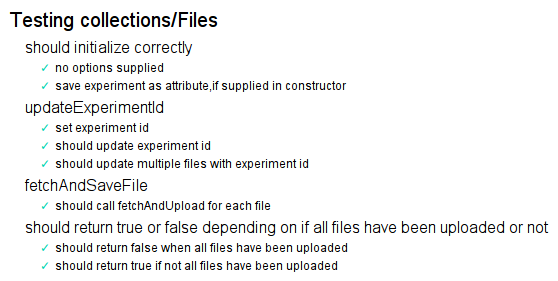
\includegraphics[width=1\textwidth]{web_test_collectionFiles.png}
\caption{The tests for the Files collection, all of which it has passed.}
\label{fig:web_test_collectionFiles}
\end{figure}

\refer{fig:web_test_collectionFiles} displays our tests of the \textit{Files} collection, checking that the collection initializes correctly, that it can update an experiment’s ID, that it can fetch and save a file, that it can check if a file has been uploaded or not.
%FIGURE X1
\begin{figure}[h]
\centering
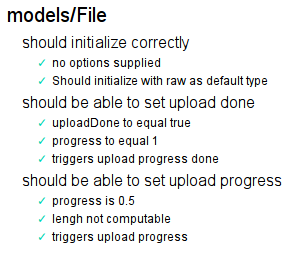
\includegraphics[width=0.6\textwidth]{web_test_modelsFile.png}
\caption{The tests for the File model, all of which it has passed.}
\label{fig:web_test_modelsFile}
\end{figure}

\refer{fig:web_test_modelsFile} displays our tests of the \textit{File} model, checking that the model initializes correctly, that it can set itself to be fully uploaded, and that it can set itself to have an upload progress (for example, a file that is halfway uploaded should set it’s progress to 0.5).
%FIGURE X2
\begin{figure}[h]
\centering
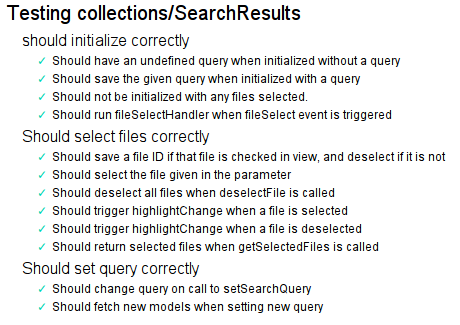
\includegraphics[width=1\textwidth]{web_test_collectionsSearchResults.png}
\caption{The tests for the SearchResults collection, all of which it has passed.}
\label{fig:web_test_collectionsSearchResults}
\end{figure}

\refer{fig:web_test_collectionsSearchResults} displays our tests of the SearchResults collection, checking that the collection initializes correctly, that it can select files correctly, that it can set a new query and that it will fetch new models upon getting a new query.
%FIGURE X3
\begin{figure}[h]
\centering

\includegraphics[width=0.6\textwidth]{web_test_modalAC.png}
\caption{The test for the ModalAC view, which it has passed.}
\label{fig:web_test_modalAC}
\end{figure}

\refer{fig:web_test_modalAC} displays the one test we have for the ModalAC view, checking that it renders it’s child when show is called.
%FIGURE X4
\begin{figure}[h]
\centering

\includegraphics[width=0.6\textwidth]{web_test_viewsMainMenu.png}
\caption{The test for the MainMenu view, which it has passed.}
\label{fig:web_test_viewsMainMenu}
\end{figure}

\refer{fig:web_test_viewsMainMenu} displays the one test we have for the MainMenu view, checking that it registers a call to render when the route changes.
\FloatBarrier

\subsection{Android}
This section focuses on the communication  between classes and how the Android application works.
\subsubsection{Login request}
	When the user starts the application and is prompted for a login, the following sequence \refer{fig:and_loginseq} of actions is performed by the system. 	\\
	
	\begin{itemize}
		\item
			User starts the application and is prompted with a login.
			Then the user-name and password is passed on to the LoginFragment.
		\item
			LoginFragment sends a login request to the ComHandler, with the user-name and password.
		\item
			The ComHandler initializes Communicator and sends a setupConnection command to verify that connection can be made. Then initializes the MsgFactory and request a login-package using the createLogin method.
		\item
			MsgFactory responds to ComHandler with a login-package in JSon format. Then the ComHandler calls the sendRequest method in Communicator with the login-package and waits for reply.
		\item
			The Communicator connects to the remote Genomizer server with a HTTP-request containing the login-package as a JSon object. If the search is valid the server will respond with code 200 and a user-token as a JSon-object.
		\item
			The JSon-object is then returned to the ComHandler which will store the token and return a boolean to the LoginFragment informing if the login was successful or not.
		\item 
			If the response was true the LoginFragment will startup the SearchFragment and present that view to the user. The Login Fragment will be terminated at that point. 
			
	\end{itemize}

	\begin{figure}[h]
		\addImageVertical{and_login_seq.jpg}
		\caption{Sequence diagram for a login-request}
		\label{fig:and_loginseq}
	\end{figure}
	
\subsubsection{Search request}
	This will display the sequence of a search request from the user to the server and back again \refer{fig:and_searchseq}.
	
	\begin{itemize}
		\item
			User will make a search request on the screen and press on the search button. That will trigger the SearchFragment to startup the ExperimentListFragment with the search string sent in as a Intent-Extra variable.
		\item
			The ExperimentListFragment will then initialize the ComHandler and call the search method with the search-list provided by the SearchFragment.
		\item
			ComHandler initializes the Communicator and determines if a connection can be made.
		\item
			If connection can be made the ComHandler initialize the MsgFactory and calls the createRegularPackage method, which will return a pre-formatted JSon-object to be used with the search request to the server.
		\item
			ComHandler calls Communicator using the sendRequest method passing on the JSon-object containing the search-list, and waits for the reply from Communicator.
		\item
			Communicator connects to the Genomizer server with a HTTP request containing a JSon object with the search-list. The server will respond with code 200 and a JSon-object with the search result from the server.
		\item
			Communicator will reconfigure the JSon object to a GenomizerHttpPackage object to preserve both the head and body from the server response. Then the GHttp-object is returned to the ComHandler.
		\item
			The ComHandler will initalize the MsgDeconstruct and send the collected JSon-object containing the search result from the server to the deconSearch method.
		\item
			MsgDeconstruct will parse the JSon-object to an ArrayList of experiments, and return that to the ComHandler.
		\item
			ComHandler will then return the search-results to the ExperimentListFragment that will present the results for the user on the screen.
	\end{itemize} 

	\begin{figure}
		\addImageVertical{and_search_seq.jpg}
		\caption{Sequence diagram for a search-request}
		\label{fig:and_searchseq}
	\end{figure}
\subsubsection{Testing}
Testing has been done successively and the foremost type of testing has been JUnit tests. Although regular running and logs have been done too.

All fragments mentioned in \ref{sec:and_classdescription} have been tested visually and through running as no viable way of unit testing them was found.

Most of the classes labeled model in \ref{sec:and_classdescription} have been tested with a test driven developlment approach, except for the small classes such as Experiment, Annotation, GeneFile and GenomizerHttpPackage as they are very straight forward (And they are indirectly shown as working through the tests of the other classes).

Most tests are run against the mockup server. Albeit some are run against the real server as the authenticity of both the methods ability to handle data as well as their ability to get a response from the real server is relevant.

\FloatBarrier

\subsection{iOS}
In the following section, details regarding the implementation of the iOS application is described using sequence diagrams and.

\subsubsection{Login}

When the user tries to log in to the system, they enter username and password and clicks on the login button. The username and password is sent to the server which validates that they are valid. If they are valid, the user is presented with the main view of the application, otherwise an error message is displayed. This sequence is shown in  \refer{fig:ios_sequence_login}.

\begin{figure}[ht]
\addImageVertical{ios_login_sequence_diagram.png}
\caption{Login sequence diagram.}
\label{fig:ios_sequence_login}
\end{figure}

\subsubsection{Search}

Once the user is logged in to the system and they have reached the main view, they can immediately start searching by selecting a number of search criteria on the screen and pressing the search button. The search criteria are converted into a valid \term{PubMed}-style query which in turn is converted into a valid \term{HTTP request} and sent to the server. The server responds with all results matching the search criteria and the results are presented to the user in a \term{SearchResultView}. This sequence is shown in \refer{fig:ios_sequence_search}.

\begin{figure}[ht]
\addImageVertical{ios_search_sequence_diagram.png}
\caption{Login sequence diagram.}
\label{fig:ios_sequence_search}
\end{figure}

\subsubsection{Experiment Selection}

In the \term{SearchResultTableView}, the user can click on an experiment to see which files are contained in an experiment. The file contents of an experiment is displayed in a \term{FileView}. The sequence is shown in \refer{fig:ios_sequence_experiment_selection} 

\begin{figure}[ht]
\addScaledImageVertical{0.5}{ios_select_experiment_sequence_diagram.png}
\caption{Experiment selection sequence diagram.}
\label{fig:ios_sequence_experiment_selection}
\end{figure}

\subsubsection{File Selection}

From the \term{FileView}, the user can select any number of files to add to a list of currently selected files by pressing the switch button next to each file name and pressing the \term{Add to Selected files} button. After that, the user can press the \term{Selected Files} button to go to the \term{Selected Files View}. This sequence is shown in \refer{fig:ios_sequence_file_selection}

\begin{figure}[ht]
\addScaledImageVertical{0.5}{ios_select_file_sequence_diagram.png}
\caption{File selection sequence diagram.}
\label{fig:ios_sequence_file_selection}
\end{figure}

\FloatBarrier

\subsubsection{Testing}

Unit-tests have been written for nearly all underlying classes. This includes JSONBuilder, ExperimentDescriber, Experiment, ExperimentFile, and ExperimentParser. These tests check all required functionality, including but not limited to proper object creation. Exactly what all the tests do is explained in the test names and comments. ServerConnection has not been tested, this is work for the next sprint. User interface functionality and integration testing has been done using exploratory methods. These tests have not been recorded or documented.

\FloatBarrier

\section{Server}
This section cointains information about implementation and tests for the different parts of the server.

\subsection{Communication}
This section explains implementation details of certain bits of the communication/control part of the system.
\subsubsection{Doorman}
The doorman is a class which handles all incoming connections and requests. The doorman reads the header and checks what kind of HTTP method it is (GET, PUT, PUSH, PULL or DELETE). A switch statement switch on these different methods.\\
\\
After switching on the different methods another switch statement is used to switch on the different types of commands, for example /experiment, /file, /search or /process. From that point a specific command object is created corresponding to the correct command, for example \textbf{GET /experiment} will create a \term{getExperimentCommand}.
\subsubsection{Command object}
The command object represent a specific command. It is created from the RESTful header and/or the JSON body sent from the client. The JSON API provides methods for automatic parsing of the JSON body into an object. The fields in the command object created must match the attributes in the JSON body. This match is case sensitive

\paragraph{Execute}
Every command object must implement a execute method. This method is the part of the command which uses the system interface to perform the task that corresponds to the command.\\
\\
The execute method returns a response object which is sent up to the doorman which then sends the response to the client. 
\paragraph{Validation}
Every command must implement a validate method. This method is run after the command is created but before the command is executed.\\
\\
The validate method returns a boolean. If the command is correctly parsed with correct data the method returns true, otherwise false. This validate is used to prevent unneccesary communication.
\subsubsection{Response object}
There are different response objects for different kind of responses since the form of the response to the client depends on the command the client initially sent.\\
\\
The response object contains all the data necessary to create a RESTful header and a JSON body for the response.
\subsubsection{Database settings}
When starting the server the database settings are set depending on the first argument of the server arguments. The argument could either be \textbf{test} or \textbf{global}.\\\\
The \textbf{test} argument will set the database settings to match a local test database, and the \textbf{global} argument will set the settings to match a global database.
\FloatBarrier

%\subsection{Conversion}
%\input{implementation/con_implementation]
\FloatBarrier

%\subsection{System administration}
%\FloatBarrier

%\subsection{Filetransfer}
%\FloatBarrier

\subsection{Database}
The following text describes the different classes the server uses to cummunicate with the database.

\subsubsection{Annotation}
When a user wants the properties of an \term{annotation} they will retrieve this object. It holds information about the data type, label, forced annotation, default value and annotation choices for drop down menus. With this object the graphical interfaces can set up a search view dynamically.

\subsubsection{Experiment}
A container of an experiments annotations and their values. The annotation labels and values are contained in a \term{hashmap} with label as key. All files corresponding to the actual experiment lies in a list of \term{FileTuple} objects.

\subsubsection{FileTuple}
A simple class that holds all information of a file in variables found in the database. Holds links for download and upload of the specific file.

\subsubsection{FilePathGenerator}
When a user wants to write or download a file, the \term{FilePathGenerator} class will take care of giving the server a file path. When a new experiment is added to the database, FPG is called and it will create a folder for the experiment and sub folders for the different file types. When a new \term{genome version} is to be added to the database, FPG will create file paths to a folder folder outside of the experiment folders. They are divided into folders corresponding to species.  This is done to give access to genome files independent of experiment id's. Chain files are given paths to sub folders within the species folders in the genome root folder.

\subsubsection{PubMedToSQLConverter}
Converts a string with \term{pubMed} notations and returns an \term{SQL query}. PubMed searches can take this shape: \texttt{raw1[FileType] AND Per[Author]} which means \term{search for all raw files that Per created}. The user enters the values with variables in a logical sequence and can add parentheses for further filtering. \term{AND}, \term{OR} and \term{NOT} are commands that can be used in the sequence. The converter can both be used for file- and experiment searches. All the variables in the pubMed string are converted to the \texttt{WHERE} section of an SQL query. When a method is called in the database API (DatabaseAccessor), the first half of the query will be combined with the one generated by the converter to form a full query. Depending on which method is called in the \term{API} (what the user wants to do), the first half of the query will vary.

\subsubsection{DatabaseAccessor}
A class that serves as API for the server for database access. It handles all connections and queries to the database. The methods simplifies queries to the database by taking as few parameters as possible to accomplish a sufficient database search. The returns of the different methods are made as simple as possible depending on the amount of data generated. If only one column is to be returned after a search, a list is sufficient. When a user wants information on several files, lists of objects will be returned with all data. \term{Prepared Statements} are created from a combination of queries and variables to avoid SQL injections. Methods that have some resemblance are grouped together for easier navigation in the API.

\subsubsection{Testing}
All methods are created with \term{Test Driven Development} (TDD). Testing is done before implementation. The better part of the testing is creating queries that gives the right results. All queries have at at least one test to verify it's functionality. The tests are run in a test suite so every method in the whole program can be tested in one run. Database methods have setup and teardown methods for setting up and resetting the database between the different tests. This is done to prevent a test to influence the result of another test.

\FloatBarrier


\begin{appendix}

\chapter{\textit{User Stories}}
\label{chap:userstories}

User stories
\chapter{\textit{Server commands}}
\label{chap:servercmd}
program: apache2\\
port: 8000\\
login: null\\
password: null\\
info: webserver http://scratchy.cs.umu.se:8000/\\
\makebox[\linewidth]{\rule{\textwidth}{0.4pt}}
program: ssh passphrase\\
port: 0\\
login: null\\
password: *****\\
info: ssh key for server in mc333, (used for git)\\
\makebox[\linewidth]{\rule{\textwidth}{0.4pt}}
program: JBDC\\
port: 0\\
login: null\\
password: null\\
info: include own jars: /usr/local/lib/psql\_jbdc4.jar\\
\makebox[\linewidth]{\rule{\textwidth}{0.4pt}}
program: postgresql database\\
port: 6000\\
login: postgres\\
password: *****\\
info: psql -h hostname -p 6000 dbname username\\
\makebox[\linewidth]{\rule{\textwidth}{0.4pt}}
program: phppgadmin\\
port: 8000\\
login: postgres\\
password: *****\\
info: http://scratchy.cs.umu.se:8000/phppgadmin use for remote psql management\\
\makebox[\linewidth]{\rule{\textwidth}{0.4pt}}
program: SSH tunnel port\\
port: 0\\
login: null\\
password: null\\
info: \%> ssh -g -R (wanted port on scratchy):(host of server):(server port) -N -f (cs-user)@scratchy.umu.se\\
\makebox[\linewidth]{\rule{\textwidth}{0.4pt}}
program: SSH to server\\
port: 2222\\
login: null\\
password: *****\\
info: ssh pvt@scratchy.cs.umu.se -p 2222\\
\makebox[\linewidth]{\rule{\textwidth}{0.4pt}}
program: host/download.php\\
port: 8000\\
login: database user\\
password: database pass\\
info: parameters: "path" - path to the file on the server. Example:\\ /var/www/data/Exp1/raw/humanarm.fastq\\
Example URL:\\ http://scratchy.cs.umu.se:8000/download.php?\\ path=/var/www/data/Exp1/raw/humanarm.fastq\\
\makebox[\linewidth]{\rule{\textwidth}{0.4pt}}
program: host/upload.php\\
port: 8000\\
login: database user\\
password: *****\\
info: parameters: "path" - path to the file on the server Example:\\ /var/www/data/Exp1/raw/humanarm.fastq\\
\chapter{\textit{Server commands}}
\label{chap:exp_app_ubuntu}
\section{Introduction}
This document will guide a user through the process to configure the server machine needed for the \appName\ server software. This guide is created while configuring a newly installed machine running Ubuntu 14.04. Other Linux or UNIX operating systems could have other commands to install different softwares. Some experience with a terminal and the UNIX environment is presumed.

Be sure to have a fully functioning Internet connection to the server machine with the possibility to direct ports to it before continuing.

Server configuration, installation and setup written by: Emil Palm (c11epm) and Eric Sjögren (c08esn)

\section{Installation and Configuration}
The server machine must run a Linux or UNIX operating system. In order to follow this guide in the easiest manner 
possible, use any Ubuntu distribution. 

\subsection{Java}
Firstly Java must be installed on the system to be able to run some of the server software. The software requires Java 1.7 or later. 

To install Java JDK open a terminal and enter following command:
\begin{verbatim}
sudo apt-get install openjdk-7-jdk
\end{verbatim}

\subsection{OpenSSH}
To be able to access the server machine remotley OpenSSH must be installed.

Enter the following command to install OpenSSH properly.
\begin{verbatim}
sudo apt-get install openssh-server openssh-client openssh-sftp-server
\end{verbatim}

\subsection{Apache2}\label{sec:exp_apache2}
In order to handle web requests and file transfering the server will use Apache2. 

To install Apache2 with necessary software, use this command:
\begin{verbatim}
sudo apt-get install apache2 apache2-utils
\end{verbatim}
After installation of Apache2 some configuration is needed. Follow the steps below.
\subsubsection{Configure listening port}\label{ports}
The default port for listening is set to 80. If this seeks to be changed follow the steps below.
\begin{enumerate}
	\item Open file with following command: \begin{verbatim}sudo nano /etc/apache2/ports.conf\end{verbatim}
    \item Edit the value in the file after ``Listen'' to the prefered port to use for listening. 
    For example: \begin{verbatim}Listen 80\end{verbatim}
    \item Save and close the file.
    \item Restart the Apache server with: \begin{verbatim}sudo service apache2 graceful\end{verbatim}
\end{enumerate}

\subsubsection{Set document root}\label{sec:exp_docroot}
The document root on the Apache server is where the root folder for the server is located. When a user is connecting to the server it will request the content from the root folder of the server.

The \appName\ server uses \textit{/var/www/} as the document root. As default for the Apache server 
the document root is set to \textit{/var/www/html/}.
To change the root folder for the Apache server, do the following steps:
\begin{enumerate}
	\item Open the configuraton file for the document root: \begin{verbatim}sudo nano /etc/apache2/sites-enabled/000-default.conf\end{verbatim}
    \item Edit the second string in the line starting with the string ``DocumentRoot'' to the root directory to be used.
    \begin{verbatim}DocumentRoot /var/www/\end{verbatim}
    \item Save and close the configuration file.
    \item Restart the Apache server: \begin{verbatim}sudo service apasche2 graceful\end{verbatim}
\end{enumerate}

After these steps the document root is changed. Please note that in step two the root directory can be set 
to something else. If these steps are followed precisely the document root will be set to \textit{/var/www/}.

\subsubsection{Add system user}\label{sec:exp_passw}
To add a system user, you first have to create a new file containing the usernames and their corresponding passwords
by using a terminal and writing:
\begin{verbatim}htpasswd -c /ect/apache2/passwords username\end{verbatim}
Change \texttt{username} to the username wanted for the new user.

This will create a password file in \textit{/etc/apache2/}. 
The path to the password file should not be accessible for the clients. 
Then you will be asked to enter the password for the user:
\begin{verbatim}
New password: mypassword
Re-type new password: mypassword
\end{verbatim}

Instead of \texttt{mypassword}, enter the password wanted for the new user.
When everything is done you will get the message:
\begin{verbatim}Adding password for user username\end{verbatim}
The passwords in the file will be stored encrypted. To add more users, the following command must be used: 
\begin{verbatim}htpasswd /ect/apache2/passwords username\end{verbatim}
If the \texttt{-c} flag is used, a new file will overwrite the old one so all users will be overwritten. For more information, see \cite{exp_apache2user} 

\subsubsection{Setup protected folders for users}\label{sec:exp_protected}
The Apache server software have functionality to make protected directories to restrict access to its content. To set this 
up it is necessary to create a user for the Apache server (\textit{read \ref{sec:exp_passw}}) to be able to access the files. 

To restrict users from accessing the folders you can make them password protected. To do this, open the file 
\textit{apache2.conf} that is located in \textit{/etc/apache2/}. In the file, new folders can be added. 
These folders will be password protected. To add a directory, new directory tags 
$<$Directory$><$/Directory$>$ must be added among the others.
A step-by-step instruction of how to password protect a folder follows:
\begin{enumerate}
	\item Open the file by the following command:
    \begin{verbatim} sudo nano /etc/apache2/apache2.conf\end{verbatim}
    \item Paste in the following in the file:
\begin{verbatim}
<Directory /path_to_document_root/path_to_restricted_folder/>
    AuthUserFile /etc/apache2/passwords
    AuthName "This is a protected area"
    AuthType Basic
   	Require valid-user
</Directory>
\end{verbatim}
Make sure that the \textit{/path\_to\_document\_root/} is set to the document root set in \ref{sec:exp_docroot}. Then \textit{path\_to\_restricted\_folder/} needed to be changed to the actual path to the folder that is to be protected. For more information see \cite{exp_apache2user}.
	\item Make sure your setup is correct.
    \item Save and close the file.
    \item Restart the Apache server to make changes:
    \begin{verbatim}sudo service apache2 graceful\end{verbatim}    
\end{enumerate}

\subsubsection{Setup restricted folders for all users}\label{sec:exp_restricted}
It is also possible to make a folder restricted for all users and only accessible through the server machine or the PHP scripts. This is done almost exactly as in \ref{sec:exp_protected}. The difference is that you add something else between the directory tags $<$Directory$><$/Directory$>$. Follow step 1 to 5 in \ref{sec:exp_protected} but instead paste this to the file at step 2:
\begin{verbatim}
<Directory /path_to_document_root/path_to_restricted_folder/>
    Require all denied
</Directory>
\end{verbatim}


\subsubsection{Setup proxy redirect}
To allow tunneling through the Apache server to the \appName\ server software, a proxy pass has to be set up.
To enable the module for Apache, enter the following command in the terminal:

\begin{verbatim}
sudo a2enmod proxy_http
\end{verbatim}
After the module is loaded a proxy pass has to be set up, the proxy pass works on a url and sends all requests to that url to the proxied address. Start by opening the file:
\begin{verbatim}
sudo nano /etc/apache2/apache2.conf
\end{verbatim}
Scroll down to the end of the file and enter this row (don't forget to modify the url and the proxy to your server setup):
\begin{verbatim}
#Proxypass 
ProxyPass /anyurlyouwant/ http://your.server.address:port/
\end{verbatim}
In this server setup this line looks like this:
\begin{verbatim}
ProxyPass /api/ http://scratchy.cs.umu.se:7000/
\end{verbatim}
This means that all requests sent to \emph{http://scratchy.cs.umu.se:8000/api/Login} will be proxyed (tunneled) to
\emph{http://scratchy.cs.umu.se:7000/Login} for example. \textbf{Do not forget to restart the Apache server}:
\begin{verbatim}
sudo service apache2 restart
\end{verbatim}
\subsection{Git}
This project uses gitHub for easy sharing of the code between all collaborators. For this to work, the server machine must have git installed to be able to clone the repositories with code. 

This document will not specify how to use git, instead please read the two guides \cite{exp_gitguide} and \cite{exp_gitguide2}

To install git on the server machine, enter the following line in the terminal:
\begin{verbatim}sudo apt-get install git\end{verbatim}
For easy access to gitHub, SSH-keys can be added to easily execute push and pull of repositories. 
See gitHub's guide \cite{exp_sshguide}.

\subsection{PHP5}
The Apache server uses PHP scripts to upload and download files. Therefore it is necessary to install PHP5 on the server machine. To install PHP5, just enter the following command in a terminal:
\begin{verbatim}sudo apt-get install php5-curl\end{verbatim}

The following file needs to be configurated \begin{verbatim}/etc/php5/apache2/php.ini\end{verbatim} with values:

\begin{verbatim}max_execution_time to 0\end{verbatim}
\begin{verbatim}max_input_time to -1\end{verbatim}
\begin{verbatim}upload_max_filesize to 0\end{verbatim}
\begin{verbatim}post_max_size to 0\end{verbatim}

\subsection{SRA Toolkit}
One of the PHP scripts will need the application SRA Toolkit installed. To install this application, enter the following in the terminal:
\begin{verbatim}sudo apt-get install sra-toolkit\end{verbatim}
This application is used to convert .sra files to .fastq files. To manually use SRA Toolkit enter the following in the terminal:
\begin{verbatim}fastq-dump /var/www/test/SRR869740.sra\end{verbatim}
This will open the SRR869740.sra file to a SRR869740.fastq file in the same directory of the original .sra file.





















\subsection{PostgreSQL}
For the server machine, PostgreSQL is required for the server to work as intended. To install PostgreSQL, enter the following command (note: the version 9.3 may vary):
\begin{verbatim}
sudo apt-get install postgresql-9.3 postgresql-client-9.3 postgresql-contrib-9.3 

\end{verbatim}

An admin account needs to be set up for the database, to do this follow these instructions:

\begin{enumerate}
\item Login to the PostgreSQL server by typing \begin{verbatim}  sudo -u postgres psql \end{verbatim}
where \texttt{postgres} is the default user for the database
\item Enter the following command while inside psql to set up a password for the user postgres:
\begin{verbatim}
ALTER ROLE postgres WITH ENCRYPTED PASSWORD password;
\end{verbatim}
and change \texttt{password} to whatever password is wanted.
\end{enumerate}

To grant access to the database from non-local machines, the following file must be changed (note: the version 9.3 may vary):
\begin{verbatim}
sudo nano /etc/postgresql/9.3/main/postgresql.conf
\end{verbatim}
Find the segment \emph{CONNECTIONS AND AUTHENTICATION} in the top part of the file and change the lines ''listen\_addresses'' and ''port'':

\begin{verbatim}
#------------------------------------------------------------------------------
# CONNECTIONS AND AUTHENTICATION
#------------------------------------------------------------------------------

# - Connection Settings -

listen_addresses = '*'          	    # what IP address(es) to listen on;
                                        # comma-separated list of addresses;
                                        # defaults to 'localhost'; use '*' for all
                                        # (change requires restart)
port = 6000                             # (change requires restart)

\end{verbatim}

Port of the server can be changed to whatever is wished. Now the access needs to be changed. To do this add the following lines to the file (note: the version 9.3 may vary): 
\begin{verbatim}
sudo nano /etc/postgresql/9.3/main/pg_hba.conf
\end{verbatim}
Make sure that there exists 2 lines that look like the following (change existing lines or add new ones):
\begin{verbatim}
# "local" is for Unix domain socket connections only
local   all             all                                     md5
# IPv4 local connections:
host    all             all             127.0.0.1/32            md5
\end{verbatim}
Restart PostgreSQL by typing:
\begin{verbatim}
sudo service postgresql restart
\end{verbatim}


\subsubsection{Clone database}
If there exists an old database that is wished to be migrated to the new database the following command can be executed on the machine where the database is presently:

\begin{verbatim}
sudo pg_dump -U dbUserName -d dbName -h localhost -p dbPort > backupfile.sql
\end{verbatim}
\begin{enumerate}
\item Change \verb+dbUserName+ to the username you have setup for PostgreSQL
\item Change \verb+dbName+ to the name of the database that is wished to be migrated
\item Change \verb+dbPort+ to the PostgreSQL port which it is setup to listen to
\item Change \verb+backupfile.sql+ to whatever filename is wished
\end{enumerate}

This creates a backup SQL file. Now transfer the file to the server where the database is migrated to and type in the following command to inject it into the database:

\begin{verbatim}
psql -U dbUserName -h localhost -d dbName -p dbPort < backupfile.sql
\end{verbatim}
\begin{enumerate}
\item Change \verb+dbUserName+ to the username you have setup for PostgreSQL
\item Change \verb+dbName+ to the name of the database that is wished to be migrated to
\item Change \verb+dbPort+ to the PostgreSQL port which it is setup to listen to
\item Change \verb+backupfile.sql+ to whatever it is named
\end{enumerate}
Restart PostgreSQL by typing:
\begin{verbatim}
sudo service postgresql restart
\end{verbatim}




\subsection{PgAdmin}\label{pgadmin}
PgAdmin is a software which provides a graphical interface towards the PostgresQL server and can be installed with following command:
\begin{verbatim}
sudo apt-get install pgadmin3
\end{verbatim}





\subsection{PhpPgAdmin}
PhpPgAdmin (\refer{fig:exp_phppgadminpic}) is a user friendly web interface that connects to the server PostgreSQL database. 
This is recommended to be installed if you are not very comfortable working with the database using the terminal 
interface or wish to only configure the database on the local server machine using PgAdmin (\ref{pgadmin}). 


\begin{figure}[htb]
\centering
\addImage{exp_phppgadmin.jpg}
\caption{PhpPgAdmin web interface}
\label{fig:exp_phppgadminpic}
\end{figure}

\subsubsection{Setup PhpPgAdmin}

Then install the required software by typing in the following command in the terminal:

\begin{verbatim}
sudo apt-get install phppgadmin
\end{verbatim}

Then this needs to be included by the Apache2 software, which is done by editing the file:

\begin{verbatim}
sudo nano /etc/apache2/apache2.conf
\end{verbatim}

and adding this line to the end of the file after the other includes:

\begin{verbatim}
#Include Phppgadmin
Include /etc/apache2/conf.d/phppgadmin
\end{verbatim}

Then we need to change the access settings to the phppgadmin via the Apache software, this is done by changing the file:

\begin{verbatim}
sudo nano /etc/apache2/conf.d/phppgadmin
\end{verbatim}
In the top part of the file a section is displayed as below:

\begin{verbatim}
order deny,allow
deny from all
allow from 127.0.0.0/255.0.0.0 ::1/128
#allow from all
\end{verbatim}
Change this section so that it looks like this:
\begin{verbatim}
order deny,allow
#deny from all
allow from 127.0.0.0/255.0.0.0 ::1/128
allow from all
\end{verbatim}

Now an account must be set up with the PhpPgAdmin. Make sure you have the \emph{htpasswd} software installed 
(comes with Apache2-utils). Then to set an account, enter the following command in the terminal:

\begin{verbatim}
sudo htpasswd -c /etc/phppgadmin/.htpasswd <username>
\end{verbatim}
Change the username to what you want the user to be called.
After that a prompt will be shown to enter a password, enter the password twice and then the account is setup.

Now the Apache server needs to be told where to look for the users. This is done by editing the file:


\begin{verbatim}
sudo nano /etc/apache2/sites-enabled/000-default.conf
\end{verbatim}
Then add this to the end of the file:

\begin{verbatim}
<Directory "/usr/share/phppgadmin">
        AuthUserFile /etc/phppgadmin/.htpasswd
        AuthName "Restricted Area"
        AuthType Basic
        require valid-user
</Directory>

\end{verbatim}

Now PhpPgAdmin needs to be told which port to connect to the PostgreSQL on (se configurations of the PostgreSQL server). %TODO ref
To do that changes needs to be made to the file:
\begin{verbatim}
sudo nano /etc/phppgadmin/config.inc.php
\end{verbatim}
Then change the following post to what corresponds to your server setup:
\begin{verbatim}
// Database port on server (5432 is the PostgreSQL default)
    $conf['servers'][0]['port'] = 6000; //place your postgreSQL port here 
    .
    .
    .

// passworded local connections.
    	$conf['extra_login_security'] = false; //True as standard

\end{verbatim}




Restart Apache and phppgadmin by typing:
\begin{verbatim}
sudo service apache2 restart
sudo service phppgadmin restart
\end{verbatim}

\chapter{\textit{Server commands}}
\label{chap:exp_app_debian}
\section{Introduction}
This document will guide a user through the process to configure the server machine needed for the \appName\ server software. This guide is created while configuring a newly installed machine running Debian 7.5 Wheezy. Other Linux or UNIX operating systems could have other commands to install different softwares. Some experience with a terminal and the UNIX environment is presumed.

Be sure to have a fully functioning Internet connection to the server machine with the possibility to direct ports to it before continuing.

Server configuration, installation and setup written by: Emil Palm (c11epm) and Eric Sjögren (c08esn)

\section{Installation and Configuration}
The server machine must run a Linux or UNIX operating system. In order to follow this guide in the easiest manner 
possible, use any Debian distribution. 


\subsection{Installation of Debian}
Since Debian is more stable for running server applications than other Linux distributions such as Ubuntu and Linux Mint, it is recommended to use any Debian release other those.
When partitioning the harddrives make sure to assign atleast 2 times the amount of ram as swap section, in our case we used 250GB. This is done to prevent the server from crashing in case the ram RAM is filled out.

The swap is a hardware RAM section that the system can dump to if the RAM is filled.

\subsection{Configure Debian repositories}
To allow the system to download software via terminal a few repositorie changes must be made.
To do this open the file:
\begin{verbatim}
sudo nano /etc/apt/sources.list
\end{verbatim}
Then the line
\begin{verbatim}
deb cdrom:[Debian GNU/Linux 7.5.0 _Wheezy_ - Official amd64 CD Binary-1 20140426-13:37]/ wheezy main
\end{verbatim}
needs to be commented away from the file to avoid errors when the system tries to fetch software from an non-exsitent cd rom. Then four repositories should be added to allow installation of softwares. Add the following lines to the end of the file:
\begin{verbatim}

deb http://ftp.acc.umu.se/debian/ wheezy-updates main
deb-src http://ftp.acc.umu.se/debian/ wheezy-updates main

deb http://ftp.acc.umu.se/debian/ wheezy main
deb-src http://ftp.acc.umu.se/debian/ wheezy main
\end{verbatim}
Try this out by typing:
\begin{verbatim}
sudo apt-get update
\end{verbatim}
and make sure there is no errors.

\subsection{Create a super user}
When Debian is installed there only exists one super user on the computer, and that is ''root''. To give other users on the system root acces and super user rights a configuratiion file must be changed, to open the file you need to login as root temporaly (this is not recommended to do for other things).

To login as root, type:
\begin{verbatim}
su
\end{verbatim}
Enter the password for the root, as setup in the installation. Then type the following to open the config file:
\begin{verbatim}
visudo
\end{verbatim}
Then add this line under the line where root is set.
\begin{verbatim}
username ALL=(ALL:ALL) ALL
\end{verbatim}
Where username is the user that will be given super user rights.

\subsection{Locales}
If there is a problem with the locales settings that looks something like this:
\begin{verbatim}

perl: warning: Setting locale failed.
perl: warning: Please check that your locale settings:
	LANGUAGE = "en_GB:en",
	LC_ALL = (unset),
	LC_COLLATE = "sv_SE",
	LC_MEASUREMENT = "sv_SE",
	LC_PAPER = "sv_SE",
	LANG = "C"
    are supported and installed on your system.
perl: warning: Falling back to the standard locale ("C").


\end{verbatim}
Try this fix:
\begin{verbatim}
export LC_ALL=en_GB.UTF-8
sudo /usr/sbin/locale-gen 
sudo dpkg-reconfigure locales
\end{verbatim}
Then reboot the server.

\subsection{Java}
Firstly Java must be installed on the system to be able to run some of the server software. The software requires Java 1.7 or later. 

To install Java JDK open a terminal and enter following command:
\begin{verbatim}
sudo apt-get install openjdk-7-jdk
\end{verbatim}

\subsection{OpenSSH}
To be able to access the server machine remotley OpenSSH must be installed.

Enter the following command to install OpenSSH properly.
\begin{verbatim}
sudo apt-get install openssh-server openssh-client openssh-sftp-server
\end{verbatim}

\subsection{Apache2}\label{sec:exp_d_apache2}
In order to handle web requests and file transfering the server will use Apache2. 

To install Apache2 with necessary software, use this command:
\begin{verbatim}
sudo apt-get install apache2 apache2-utils
\end{verbatim}
After installation of Apache2 some configuration is needed. Follow the steps below.
\subsubsection{Configure listening port}\label{sec:exp_d_ports}
The default port for listening is set to 80. If this seeks to be changed follow the steps below.
\begin{enumerate}
	\item Open file with following command: \begin{verbatim}sudo nano /etc/apache2/ports.conf\end{verbatim}
    \item Edit the value in the file after ``Listen'' to the prefered port to use for listening. 
    For example: \begin{verbatim}Listen 80\end{verbatim}
    \item Save and close the file.
    \item Restart the Apache server with: \begin{verbatim}sudo service apache2 graceful\end{verbatim}
\end{enumerate}

\subsubsection{Set document root}\label{sec:exp_d_docroot}
The document root on the Apache server is where the root folder for the server is located. When a user is connecting to the server it will request the content from the root folder of the server.

The \appName\ server uses \textit{/var/www/} as the document root. As default for the Apache server 
the document root is set to \textit{/var/www/html/}.
To change the root folder for the Apache server, do the following steps:
\begin{enumerate}
	\item Open the configuraton file for the document root: \begin{verbatim}sudo nano /etc/apache2/sites-enabled/000-default.conf\end{verbatim}
    \item Edit the second string in the line starting with the string ``DocumentRoot'' to the root directory to be used.
    \begin{verbatim}DocumentRoot /var/www/\end{verbatim}
    \item Save and close the configuration file.
    \item Restart the Apache server: \begin{verbatim}sudo service apasche2 graceful\end{verbatim}
\end{enumerate}

After these steps the document root is changed. Please note that in step two the root directory can be set 
to something else. If these steps are followed precisely the document root will be set to \textit{/var/www/}.

\subsubsection{Add system user}\label{sec:exp_d_passw}
To add a system user, you first have to create a new file containing the usernames and their corresponding passwords
by using a terminal and writing:
\begin{verbatim}htpasswd -c /ect/apache2/passwords username\end{verbatim}
Change \texttt{username} to the username wanted for the new user.

This will create a password file in \textit{/etc/apache2/}. 
The path to the password file should not be accessible for the clients. 
Then you will be asked to enter the password for the user:
\begin{verbatim}
New password: mypassword
Re-type new password: mypassword
\end{verbatim}

Instead of \texttt{mypassword}, enter the password wanted for the new user.
When everything is done you will get the message:
\begin{verbatim}Adding password for user username\end{verbatim}
The passwords in the file will be stored encrypted. To add more users, the following command must be used: 
\begin{verbatim}htpasswd /ect/apache2/passwords username\end{verbatim}
If the \texttt{-c} flag is used, a new file will overwrite the old one so all users will be overwritten. For more information, see \cite{exp_apache2user} 

\subsubsection{Setup protected folders for users}\label{sec:exp_d_protected}
The Apache server software have functionality to make protected directories to restrict access to its content. To set this 
up it is necessary to create a user for the Apache server (\textit{see \ref{sec:exp_d_passw}}) to be able to access the files. 

To restrict users from accessing the folders you can make them password protected. To do this, open the file 
\textit{apache2.conf} that is located in \textit{/etc/apache2/}. In the file, new folders can be added. 
These folders will be password protected. To add a directory, new directory tags 
$<$Directory$><$/Directory$>$ must be added among the others.
A step-by-step instruction of how to password protect a folder follows:
\begin{enumerate}
	\item Open the file by the following command:
    \begin{verbatim} sudo nano /etc/apache2/apache2.conf\end{verbatim}
    \item Paste in the following in the file:
\begin{verbatim}
<Directory /path_to_document_root/path_to_restricted_folder/>
    AuthUserFile /etc/apache2/passwords
    AuthName "This is a protected area"
    AuthType Basic
   	Require valid-user
</Directory>
\end{verbatim}
Make sure that the \textit{/path\_to\_document\_root/} is set to the document root set in \ref{sec:exp_d_docroot}. Then \textit{path\_to\_restricted\_folder/} needed to be changed to the actual path to the folder that is to be protected. For more information see \cite{exp_apache2user}.
	\item Make sure your setup is correct.
    \item Save and close the file.
    \item Restart the Apache server to make changes:
    \begin{verbatim}sudo service apache2 graceful\end{verbatim}    
\end{enumerate}

\subsubsection{Setup restricted folders for all users}\label{sec:exp_d_restricted}
It is also possible to make a folder restricted for all users and only accessible through the server machine or the PHP scripts. This is done almost exactly as in \ref{sec:exp_d_protected}. The difference is that you add something else between the directory tags $<$Directory$><$/Directory$>$. Follow step 1 to 5 in \ref{sec:exp_d_protected} but instead paste this to the file at step 2:
\begin{verbatim}
<Directory /path_to_document_root/path_to_restricted_folder/>
    Require all denied
</Directory>
\end{verbatim}


\subsubsection{Setup proxy redirect}
To allow tunneling through the Apache server to the \appName\ server software, a proxy pass has to be set up.
To enable the module for Apache, enter the following command in the terminal:

\begin{verbatim}
sudo a2enmod proxy_http
\end{verbatim}
After the module is loaded a proxy pass has to be set up, the proxy pass works on a url and sends all requests to that url to the proxied address. Start by opening the file:
\begin{verbatim}
sudo nano /etc/apache2/apache2.conf
\end{verbatim}
Scroll down to the end of the file and enter this row (don't forget to modify the url and the proxy to your server setup):
\begin{verbatim}
#Proxypass 
ProxyPass /anyurlyouwant/ http://your.server.address:port/
\end{verbatim}
In this server setup this line looks like this:
\begin{verbatim}
ProxyPass /api/ http://scratchy.cs.umu.se:7000/
\end{verbatim}
This means that all requests sent to \emph{http://scratchy.cs.umu.se:8000/api/Login} will be proxyed (tunneled) to
\emph{http://scratchy.cs.umu.se:7000/Login} for example. \textbf{Do not forget to restart the Apache server}:
\begin{verbatim}
sudo service apache2 restart
\end{verbatim}

To allow apache to upload and download files to the system a user called ''www-data'' must be added to the group of the user created for the system. If you dont remember what user you have setup you can write:

\begin{verbatim}
groups
\end{verbatim}
The group name should be present there. now type the following line in the terminal:

\begin{verbatim}
sudo gpasswd -a www-data groupname
\end{verbatim}
where groupname is the user you have setup for the system.

\subsection{Git}
This project uses gitHub for easy sharing of the code between all collaborators. For this to work, the server machine must have git installed to be able to clone the repositories with code. 

This document will not specify how to use git, instead please read the two guides \cite{exp_gitguide} and \cite{exp_gitguide2}

To install git on the server machine, enter the following line in the terminal:
\begin{verbatim}sudo apt-get install git\end{verbatim}
For easy access to gitHub, SSH-keys can be added to easily execute push and pull of repositories. 
See gitHub's guide \cite{exp_sshguide}.

\subsection{PHP5}
The Apache server uses PHP scripts to upload and download files. Therefore it is necessary to install PHP5 on the server machine. To install PHP5, just enter the following command in a terminal:
\begin{verbatim}sudo apt-get install php5-curl\end{verbatim}

The following file needs to be configurated \begin{verbatim}/etc/php5/apache2/php.ini\end{verbatim} with values:

\begin{verbatim}/etc/php5/apache2filter/php.ini\end{verbatim}

\begin{verbatim}max_execution_time to 0\end{verbatim}
\begin{verbatim}max_input_time to -1\end{verbatim}
\begin{verbatim}upload_max_filesize to 0\end{verbatim}
\begin{verbatim}post_max_size to 0\end{verbatim}

\subsection{SRA Toolkit}
One of the PHP scripts will need the application SRA Toolkit installed. To install this application, enter the following in the terminal:
\begin{verbatim}sudo apt-get install sra-toolkit\end{verbatim}
This application is used to convert .sra files to .fastq files. To manually use SRA Toolkit enter the following in the terminal:
\begin{verbatim}fastq-dump /var/www/test/SRR869740.sra\end{verbatim}
This will open the SRR869740.sra file to a SRR869740.fastq file in the same directory of the original .sra file.

\subsection{PostgreSQL}
For the server machine, PostgreSQL is required for the server to work as intended. To install PostgreSQL, enter the following command (note: the version 9.3 may vary):
\begin{verbatim}
sudo apt-get install postgresql-9.3 postgresql-client-9.3 postgresql-contrib-9.3 

Debian:
sudo apt-get install postgresql-9.1 postgresql-client-9.1 postgresql-contrib-9.1
\end{verbatim}

An admin account needs to be set up for the database, to do this follow these instructions:

\begin{enumerate}
\item Login to the PostgreSQL server by typing \begin{verbatim}  sudo -u postgres psql \end{verbatim}
where \texttt{postgres} is the default user for the database
\item Enter the following command while inside psql to set up a password for the user postgres:
\begin{verbatim}
ALTER ROLE postgres WITH ENCRYPTED PASSWORD 'password';
\end{verbatim}
and change \texttt{password} to whatever password is wanted.
\end{enumerate}

To grant access to the database from non-local machines, the following file must be changed (note: the version 9.3 may vary):
\begin{verbatim}
sudo nano /etc/postgresql/9.3/main/postgresql.conf
\end{verbatim}
Find the segment \emph{CONNECTIONS AND AUTHENTICATION} in the top part of the file and change the lines ''listen\_addresses'' and ''port'':

\begin{verbatim}
#------------------------------------------------------------------------------
# CONNECTIONS AND AUTHENTICATION
#------------------------------------------------------------------------------

# - Connection Settings -

listen_addresses = '*'          	    # what IP address(es) to listen on;
                                        # comma-separated list of addresses;
                                        # defaults to 'localhost'; use '*' for all
                                        # (change requires restart)
port = 6000                             # (change requires restart)

\end{verbatim}

Port of the server can be changed to whatever is wished. Now the access needs to be changed. To do this add the following lines to the file (note: the version 9.3 may vary): 
\begin{verbatim}
sudo nano /etc/postgresql/9.3/main/pg_hba.conf
\end{verbatim}
Make sure that there exists 2 lines that look like the following (change existing lines or add new ones):
\begin{verbatim}
# "local" is for Unix domain socket connections only
local   all             all                                     md5
# IPv4 local connections:
host    all             all             127.0.0.1/32            md5
\end{verbatim}
Restart PostgreSQL by typing:
\begin{verbatim}
sudo service postgresql restart
\end{verbatim}


\subsubsection{Clone database}
If there exists an old database that is wished to be migrated to the new database the following command can be executed on the machine where the database is presently:

\begin{verbatim}
sudo pg_dump -U dbUserName -d dbName -h localhost -p dbPort > backupfile.sql
\end{verbatim}
\begin{enumerate}
\item Change \verb+dbUserName+ to the username you have setup for PostgreSQL
\item Change \verb+dbName+ to the name of the database that is wished to be migrated
\item Change \verb+dbPort+ to the PostgreSQL port which it is setup to listen to
\item Change \verb+backupfile.sql+ to whatever filename is wished
\end{enumerate}

This creates a backup SQL file. Now transfer the file to the server where the database is migrated to and type in the following command to inject it into the database:

\begin{verbatim}
psql -U dbUserName -h localhost -d dbName -p dbPort < backupfile.sql
\end{verbatim}
\begin{enumerate}
\item Change \verb+dbUserName+ to the username you have setup for PostgreSQL
\item Change \verb+dbName+ to the name of the database that is wished to be migrated to
\item Change \verb+dbPort+ to the PostgreSQL port which it is setup to listen to
\item Change \verb+backupfile.sql+ to whatever it is named
\end{enumerate}
Restart PostgreSQL by typing:
\begin{verbatim}
sudo service postgresql restart
\end{verbatim}




\subsection{PgAdmin}\label{sec:exp_d_pgadmin}
PgAdmin is a software which provides a graphical interface towards the PostgresQL server and can be installed with following command:
\begin{verbatim}
sudo apt-get install pgadmin3
\end{verbatim}





\subsection{PhpPgAdmin}
PhpPgAdmin (\refer{fig:exp_d_phppgadminpic}) is a user friendly web interface that connects to the server PostgreSQL database. 
This is recommended to be installed if you are not very comfortable working with the database using the terminal 
interface or wish to only configure the database on the local server machine using PgAdmin (\ref{sec:exp_d_pgadmin}). 


\begin{figure}[htb]
\centering
\addImage{phppgadmin.jpg}
\caption{PhpPgAdmin web interface}
\label{fig:exp_d_phppgadminpic}
\end{figure}

\subsubsection{Setup PhpPgAdmin}

Then install the required software by typing in the following command in the terminal:

\begin{verbatim}
sudo apt-get install phppgadmin
\end{verbatim}

Then this needs to be included by the Apache2 software, which is done by editing the file:

\begin{verbatim}
sudo nano /etc/apache2/apache2.conf
\end{verbatim}

and adding this line to the end of the file after the other includes:

\begin{verbatim}
#Include Phppgadmin
Include /etc/apache2/conf.d/phppgadmin
\end{verbatim}

Then we need to change the access settings to the phppgadmin via the Apache software, this is done by changing the file:

\begin{verbatim}
sudo nano /etc/apache2/conf.d/phppgadmin
\end{verbatim}
In the top part of the file a section is displayed as below:

\begin{verbatim}
order deny,allow
deny from all
allow from 127.0.0.0/255.0.0.0 ::1/128
#allow from all
\end{verbatim}
Change this section so that it looks like this:
\begin{verbatim}
order deny,allow
#deny from all
allow from 127.0.0.0/255.0.0.0 ::1/128
allow from all
\end{verbatim}

Now an account must be set up with the PhpPgAdmin. Make sure you have the \emph{htpasswd} software installed 
(comes with Apache2-utils). Then to set an account, enter the following command in the terminal:

\begin{verbatim}
sudo htpasswd -c /etc/phppgadmin/.htpasswd <username>
\end{verbatim}
Change the username to what you want the user to be called.
After that a prompt will be shown to enter a password, enter the password twice and then the account is setup.

Now the Apache server needs to be told where to look for the users. This is done by editing the file:


\begin{verbatim}
sudo nano /etc/apache2/sites-enabled/000-default.conf
\end{verbatim}
Then add this to the end of the file:

\begin{verbatim}
<Directory "/usr/share/phppgadmin">
        AuthUserFile /etc/phppgadmin/.htpasswd
        AuthName "Restricted Area"
        AuthType Basic
        require valid-user
</Directory>

\end{verbatim}

Now PhpPgAdmin needs to be told which port to connect to the PostgreSQL on (se configurations of the PostgreSQL server). %TODO ref
To do that changes needs to be made to the file:
\begin{verbatim}
sudo nano /etc/phppgadmin/config.inc.php
\end{verbatim}
Then change the following post to what corresponds to your server setup:
\begin{verbatim}
// Database port on server (5432 is the PostgreSQL default)
    $conf['servers'][0]['port'] = 6000; //place your postgreSQL port here 
    .
    .
    .

// passworded local connections.
    	$conf['extra_login_security'] = false; //True as standard

\end{verbatim}




Restart Apache and phppgadmin by typing:
\begin{verbatim}
sudo service apache2 restart
sudo service phppgadmin restart
\end{verbatim}
\end{appendix}
\begin{thebibliography}{10} 

\bibitem{exp_apache2user} Authentication and Authorization \\
\url{http://httpd.apache.org/docs/2.2/howto/auth.html}
\bibitem{exp_gitguide} git - the simple guide \\
\url{http://rogerdudler.github.io/git-guide/}
\bibitem{exp_gitguide2} Git for beginners: The definitive practical guide \\
\url{http://stackoverflow.com/questions/315911/git-for-beginners-the-definitive-practical-guide}
\bibitem{exp_sshguide} Generating SSH Keys \\
\url{https://help.github.com/articles/generating-ssh-keys}

\bibitem{web_1} Backbone.js documentation: \url{http://backbonejs.org/} Retrieved 8/5 -14 
\bibitem{web_2} Bootstrap documentation: \url{http://getbootstrap.com/} Retrieved 8/5 -14 
\bibitem{web_3} AJAX on wiki: \url{http://en.wikipedia.org/wiki/Ajax_(programming)} Retrieved 8/5 -14 
\bibitem{web_4} JSON on wiki: \url{ http://en.wikipedia.org/wiki/JSON} Retrieved 8/5 -14 
\bibitem{web_5} RequireJS documentation: \url{http://requirejs.org/} Retrieved 8/5 -14 
\bibitem{web_6} JQuery documentation: \url{http://jquery.com/}  Retrieved 8/5 -14 
\bibitem{web_7} Chai documentation: \url{http://chaijs.com/} Retrieved 9/5 -14 
\bibitem{web_8} Mocha documentation: \url{http://visionmedia.github.io/mocha/} Retrieved 9/5 -14 
\bibitem{web_9} Sinon documentation: \url{http://sinonjs.org/} Retrieved 9/5 -14 

\end{thebibliography}



\end{document}